\chapter{Experiments and Results} \label{experiment_reuslts}

As mentioned earlier, the work presented in this thesis is prepared on simulation and validated on real micro UAV robot. More details about the environment of the simulation is found in \ref{simu}, and about the real robot in \ref{real_robot}. An abstraction for the real robot's hardware and software specifications are mentioned in \ref{real_robot_hardware}. Robotics Operating System (ROS) has been used because of its advantages that will be discussed in section \ref{ROS_part}.

\section{Robotics Operating System} \label{ROS_part}
In the past years ROS has proved its value and grown great attention in both research and industry since it is first introduced by Andrew Ng. et al. in 2009 \cite{quigley2009ros}. It is an open source message oriented middleware with publisher subscriber message passing process. Collaborators from many companies and research laboratories develop packages and tools with the concept of being reusable. 

% some are generic with no restriction of the hardware used. 


There are now mature enough tutorials, that can give extensive and deep view of ROS like for example technical books that show step by step development using ROS as in \cite{o2014gentle,joseph2015mastering}. It is chosen and preferred because it can be connected to various simulators and hardware.



\section{Simulation} \label{simu}
There are variety of robotics simulations available in the field nowadays like MORSE, Gazebo, V-REP,Stage, etc. Available comparison between them can be found examined by Gonçalo Nuno in \cite{augusto2013robotteamsim}.
\vfill
\hfill
% Some applications that utilize ROS and V-REP environment in their research as in \cite{olivares2014v}

\subsection{VREP}
Virtual Robot Experimentation Platform (V-REP) is introduced in 2013 by E. Rohmer et al. in \cite{rohmer2013v}. It has great advantage in speeding up the process of algorithm's development visualization and validation. The robot simulator V-REP, model can be individually controlled via an embedded script, a plugin, a ROS node, a remote API client, or a custom solution. This makes V-REP very versatile and ideal for multi-robot applications. Controllers can be written in C/C++, Python, Matlab, and more.
\vfill
\hfill

\subsubsection{Room representation}
\hfill

Several rooms were built in V-REP to act as different room scenarios. In the figure \ref{fig:final_room}(a) the black and orange parts are not areas of interest to cover. while in figure \ref{fig:final_room}(b) the red blocks are the areas of least interest.

\begin{figure}[!htb]
  \centering
  \subfigure[Small Room]{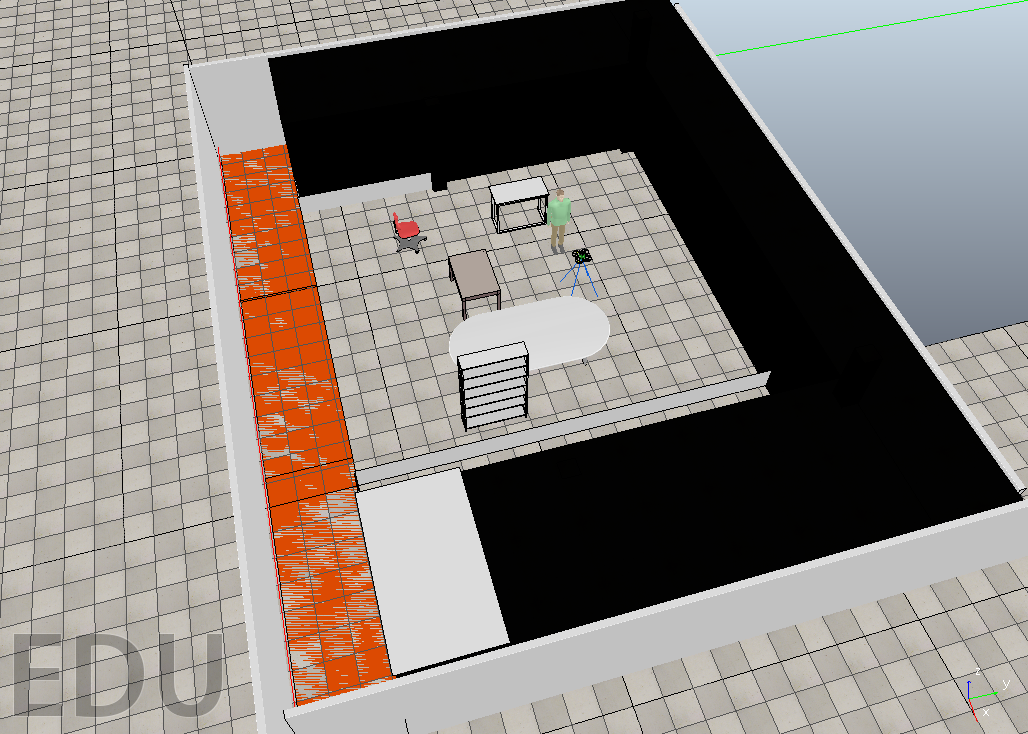
\includegraphics[width=0.55\textwidth]{figures/Room_2.png}}
  \hfill
  \subfigure[Big room]{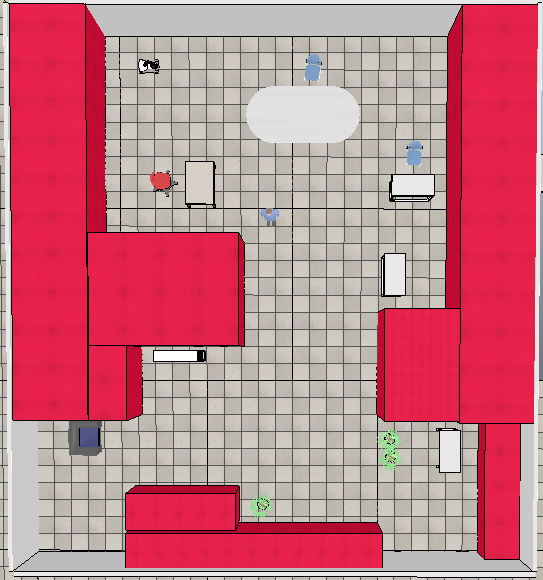
\includegraphics[width=0.42\textwidth]{figures/room_full.png}}
  \caption{Room Coverage}
  
  \label{fig:final_room}
\end{figure}

The size of the big room is 15*14 $meters^{2}$ . 


\subsection{UAV Simulation}
\begin{figure}[H]

  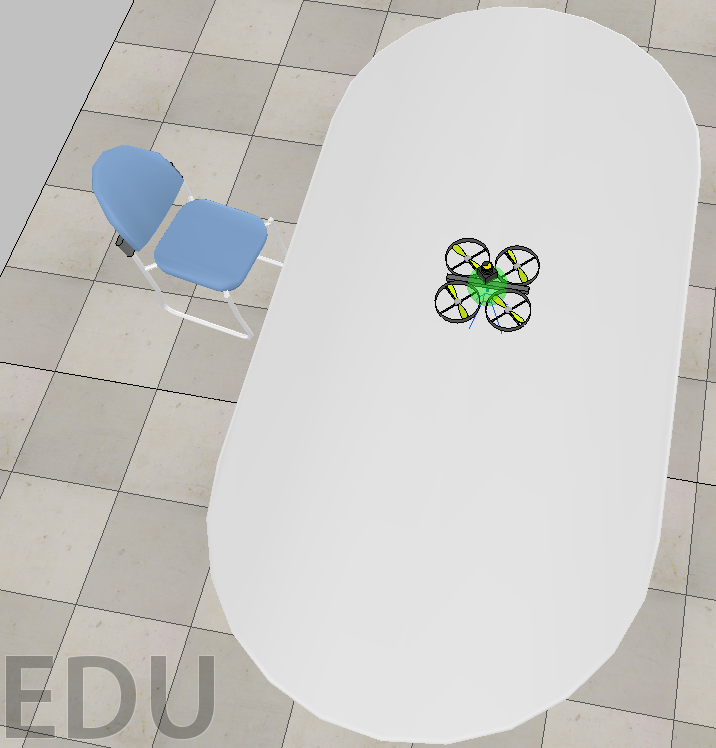
\includegraphics[width=0.5\textwidth]{figures/Drone_VREP.png}
  \caption{Drone available in V-REP with some modifications}
  
  \label{fig:drone_vrep}  
\end{figure}


\subsubsection{UAV model}

The UAV used either in simulation or real world experimentation is of micro aerial quadcopter drone like in figure \ref{fig:drone_vrep}. Obviously from the name comes quad which is implying to have 4 blade rotors. The quadcopter is controlled by adjusting the angular velocities of the rotors which are spun by electric motors. It has simpler structure compared to the other rotor crafts like helicopter. It can easily take off and land with vertical take-off and landing (VTOL). Some modifications is done on the provided model by V-REP like adding LIDAR sensor over the robot. So that in the future work, dynamic obstacle avoidance will be taken into consideration. Also a proportional-integrator-differentiator (PID) control is provided for the motors, in order to have more precise motions.
% REF : http://sal.aalto.fi/publications/pdf-files/eluu11_public.pdf


%Twist message mathematical can be found in lecture 7 graph\_slam of visual navigation for flying robots .. slide 50

\subsubsection{Mounted Camera}

There are two cameras mounted on the quadcopter available with V-REP, unfortunately their images can not be transmitted over the package used in ROS to transport and process images. For this purpose editing the available model by mounting what is called according to V-REP, vision sensor. This vision sensor is giving many properties to be edited like clipping plane distance, perspective angle, resolution and more. 

% \begin{figure}
%   \centering
%   \subfigure[Small Room]{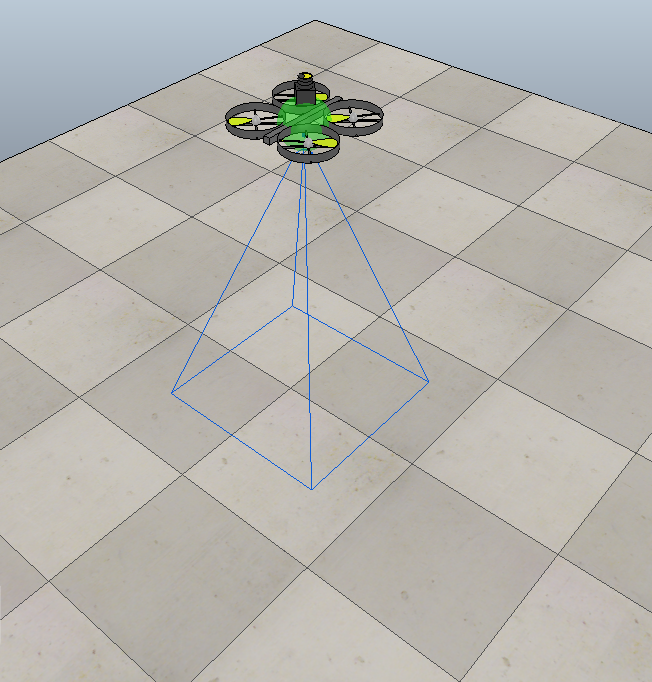
\includegraphics[width=0.23\textwidth]{figures/1m_height.png}}
%   \hfill
%   \subfigure[Big room]{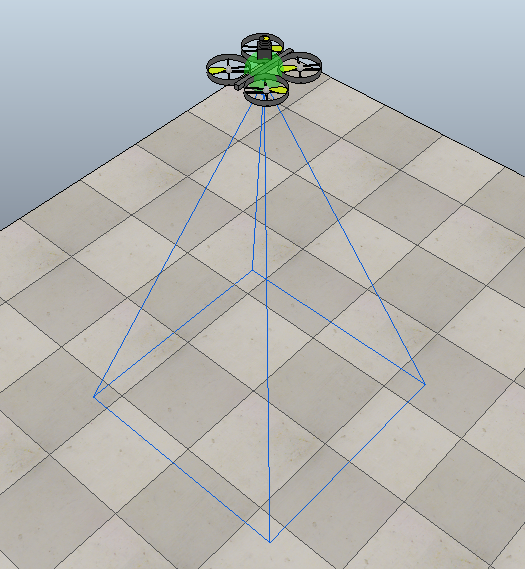
\includegraphics[width=0.23\textwidth]{figures/2m_height.png}}
  
%   \label{fig:2m_height}
%   \hfill
%   \subfigure[Big room]{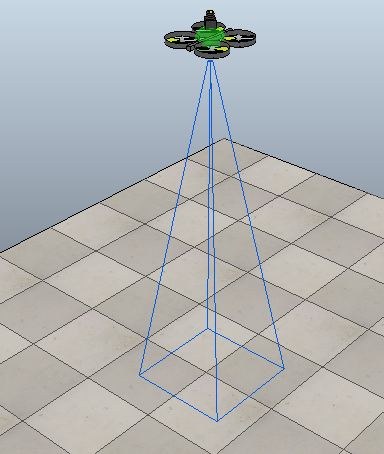
\includegraphics[width=0.23\textwidth]{figures/2m_height_small_clipping.png}}

%   \label{fig:2m_height}
  
%   \caption{Room Coverage}
% \end{figure}

% \begin{figure}[!htb]
% \minipage{0.32\textwidth}
%   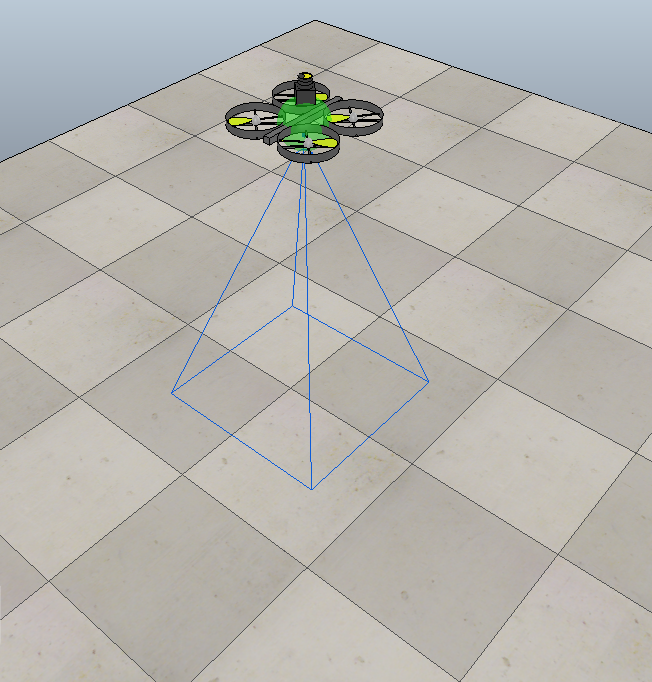
\includegraphics[width=\linewidth]{figures/1m_height.png}
%   \caption{A really Awesome Image}\label{fig:awesome_image1}
% \endminipage\hfill
% \minipage{0.32\textwidth}
%   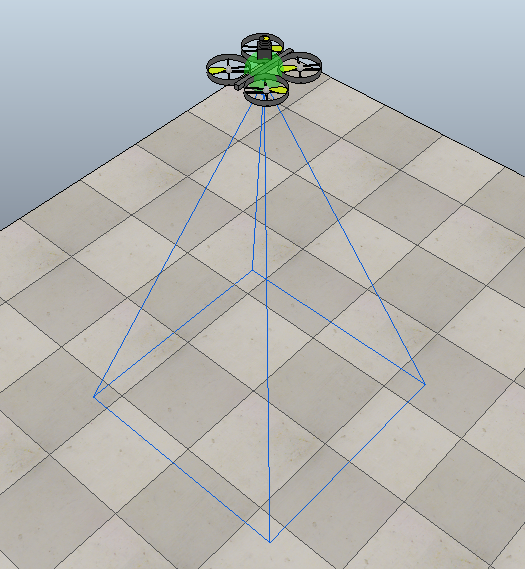
\includegraphics[width=\linewidth]{figures/2m_height.png}
% \endminipage\hfill
% \minipage{0.32\textwidth}%
%   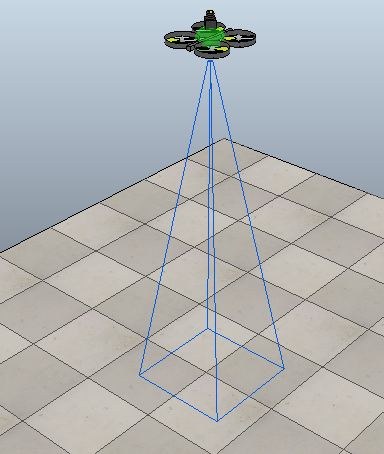
\includegraphics[width=\linewidth]{figures/2m_height_small_clipping.png}
% \endminipage
% \end{figure}

%\textcolor{red}{CLEAN THE IMAGES TO BE OF THE SAME CONTOUR}

\begin{figure}[H]
\centering
\subfigure[1m height, wide angle]{
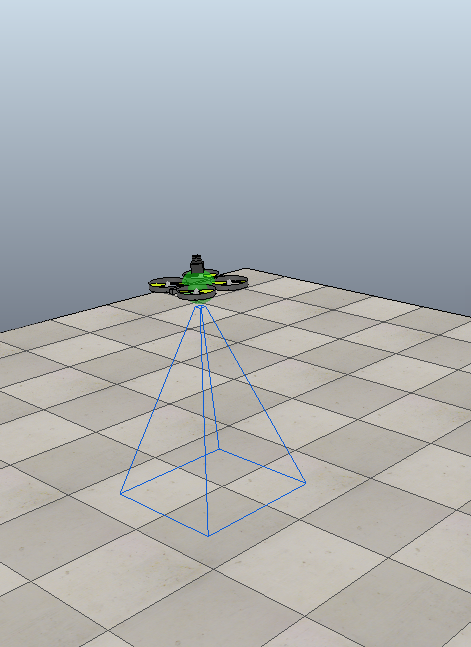
\includegraphics[width=.31\textwidth]{figures/1m36.png}
}
\subfigure[2m height, wide angle]{
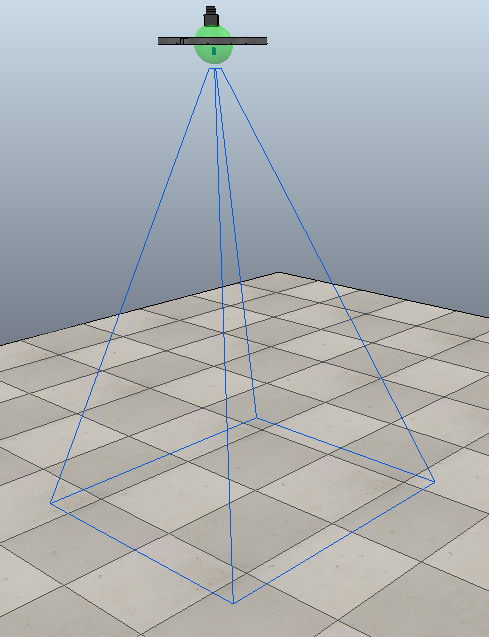
\includegraphics[width=.31\textwidth]{figures/2m36.png}
}
\subfigure[2m height, small angle]{
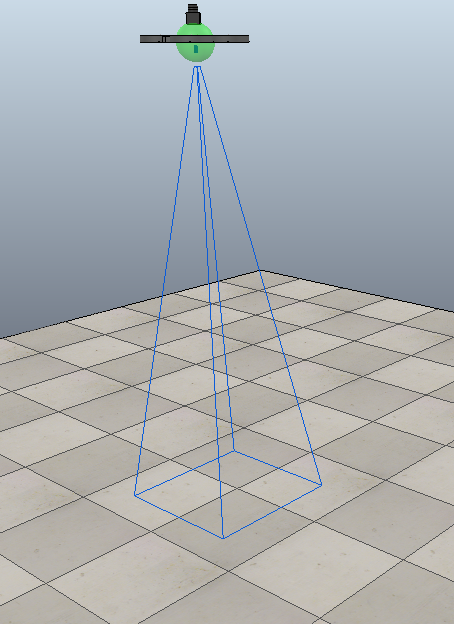
\includegraphics[width=.31\textwidth]{figures/2m18.png}
}
The previous figure is showing the change in the field of view and its effect on the captured image. This is also affecting the number of waypoints as mentioned before.

\caption{Camera projection on the ground}
\label{fig:cam_proj_vrep}
\end{figure}

\subsection{Simulation Results}
In this subsection the results generated from GA solving the TSP followed by either the linear, or spline piecewise function. Afterwards the artificial potential field results are shown. 

Results generated by using 18 waypoints, providing 79\% of area coverage.
\begin{figure}[h]
\minipage{0.334\textwidth}
  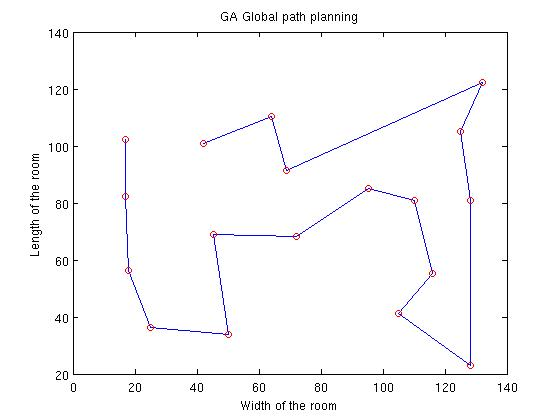
\includegraphics[width=\linewidth]{figures/18pts_GA_linear_2D.jpg}  
  \endminipage \hfill
  \minipage{0.33\textwidth}
  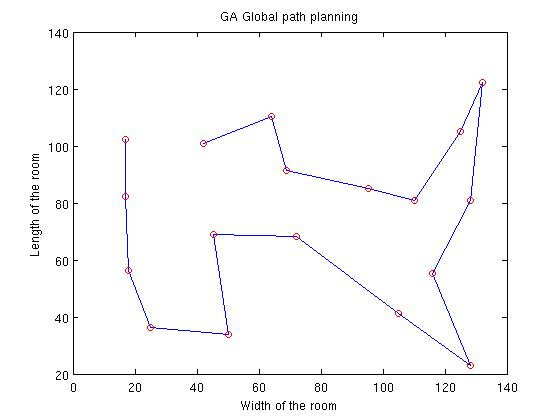
\includegraphics[width=\linewidth]{figures/18pts_GA_linear_2D_2.jpg}  
  \endminipage \hfill
  \minipage{0.33\textwidth}
  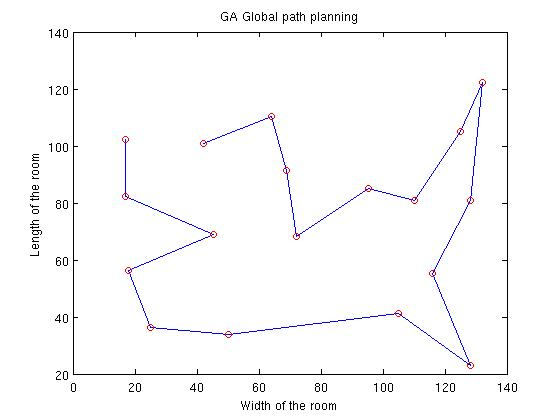
\includegraphics[width=\linewidth]{figures/18pts_GA_linear_2D_3.jpg}  
  \endminipage
  \caption{GA path planning followed by linear piecewise of 18 waypoints to cover 79\% of an area}
  \label{fig:Path_planning_linear_18}
\end{figure}

\begin{figure}[h]
\minipage{0.334\textwidth}
  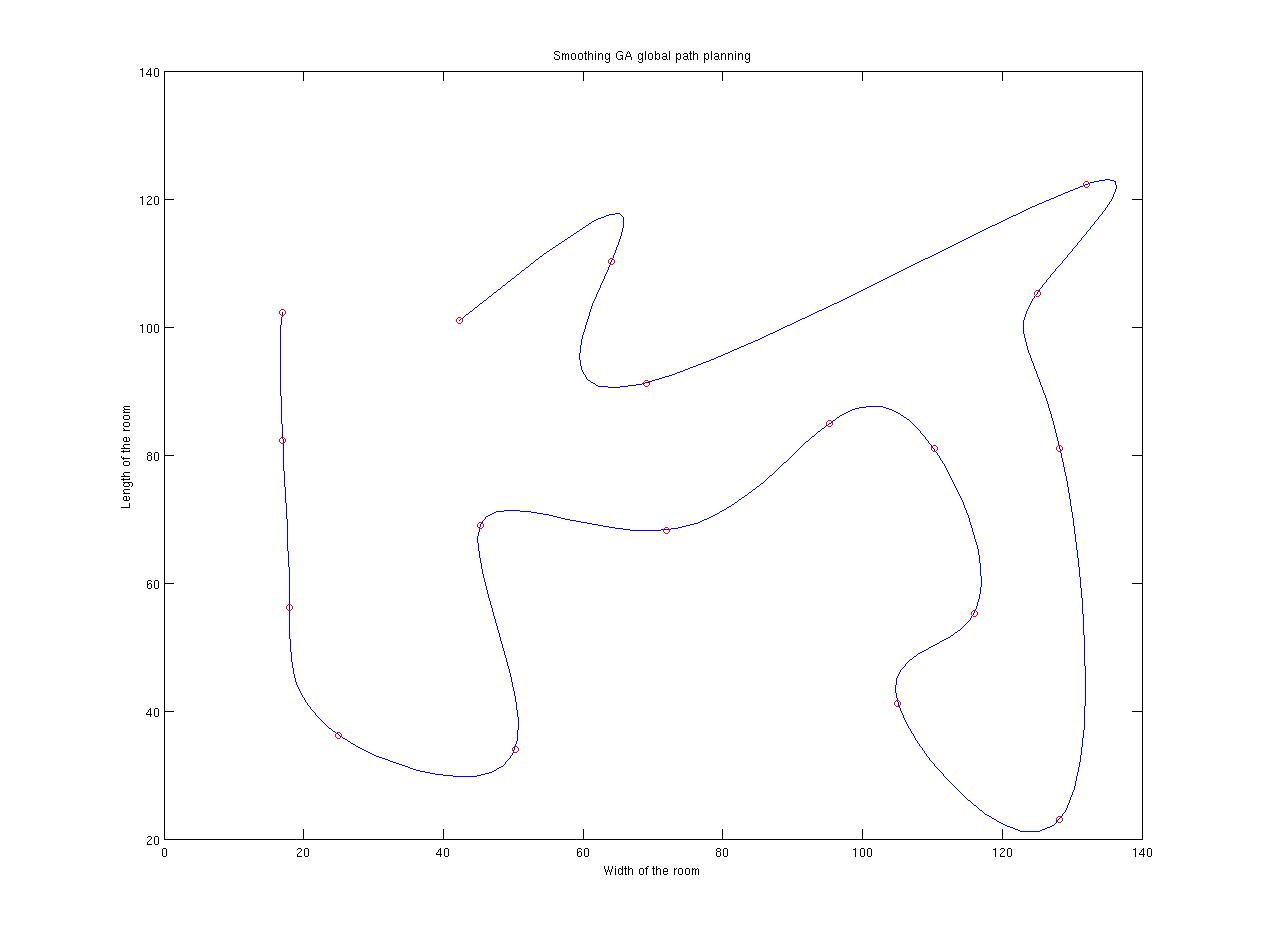
\includegraphics[width=\linewidth]{figures/18pts_GA_linear_2D_1_smooth.jpg}  
  \endminipage \hfill
  \minipage{0.33\textwidth}
  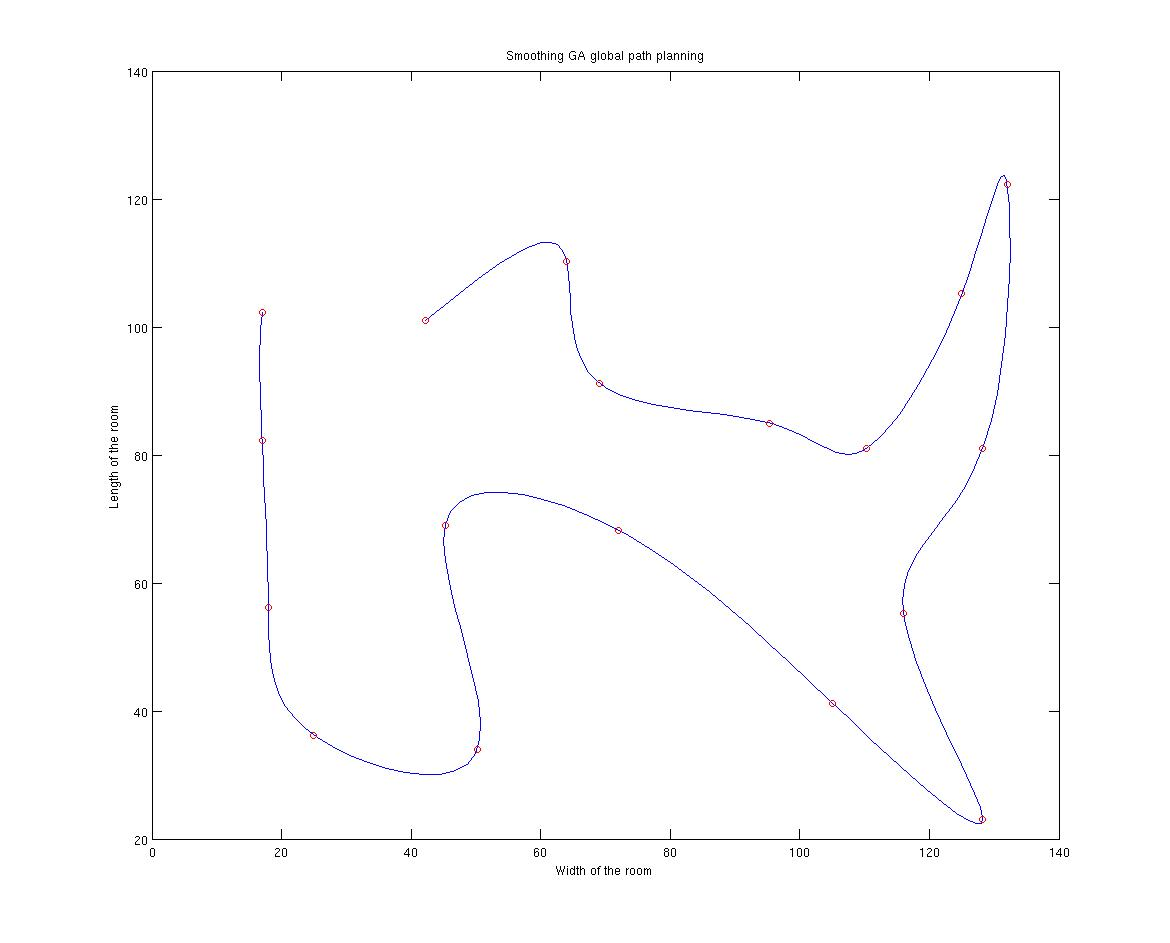
\includegraphics[width=\linewidth]{figures/18pts_GA_linear_2D_2_smooth.jpg}  
  \endminipage \hfill
  \minipage{0.33\textwidth}
  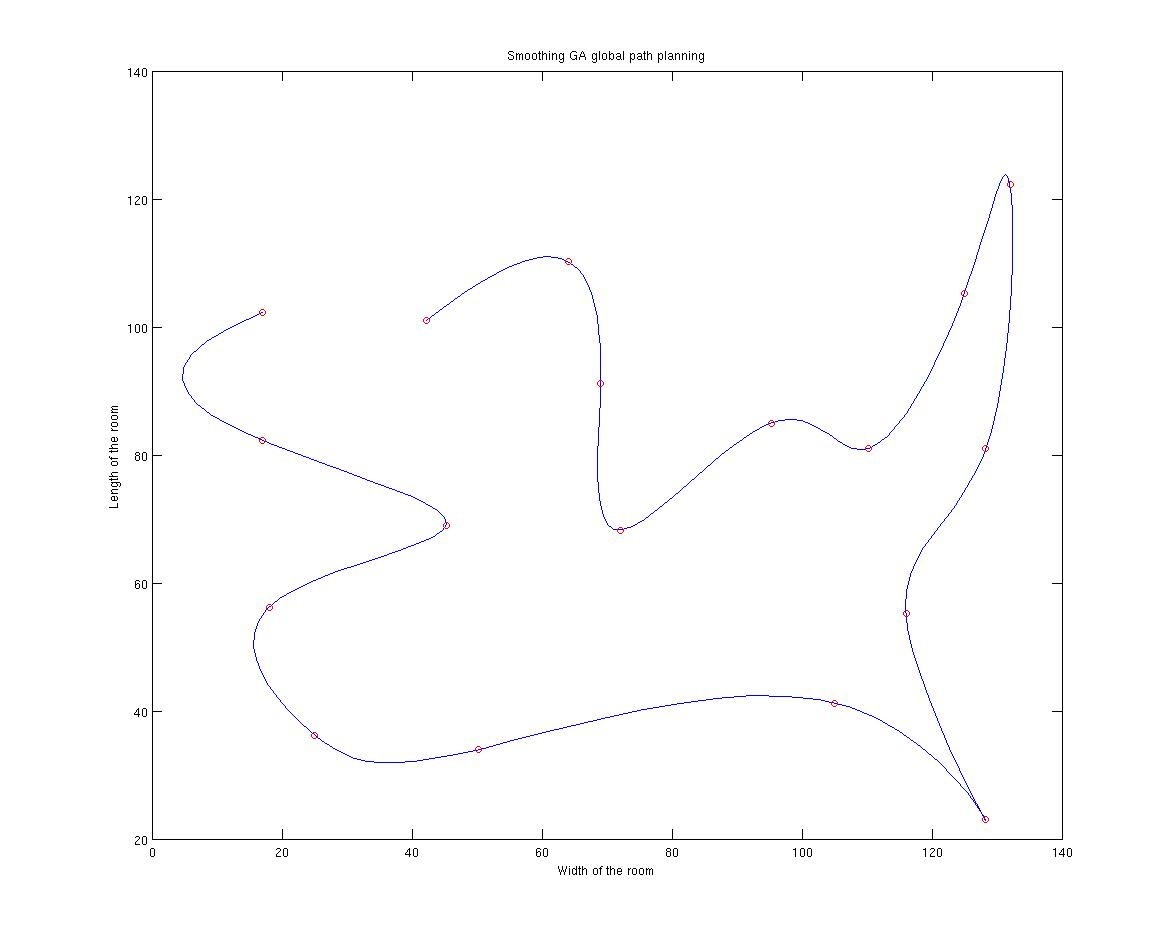
\includegraphics[width=\linewidth]{figures/18pts_GA_linear_2D_3_smooth.jpg}  
  \endminipage
  \caption{Smoothing GA path planning of 18 waypoints to cover 79\% of an area}
  \label{fig:smooth_ga_18}
\end{figure}

\hfill

The results shown in the previous paths are generated with the same parameters specification of the GA with letting the starting node to be anywhere inside the arena. The left path length is 486 meters, the middle path is 463.4714 meters, while the right one is 474 meters for the same area coverage percentage. There are variations of results because GA acquires randomness in finding the solution. This randomness appears in the evolution of the populations ( proposed tours in the iterations) of the program.

\begin{figure}[H]
\minipage{0.50\textwidth}
  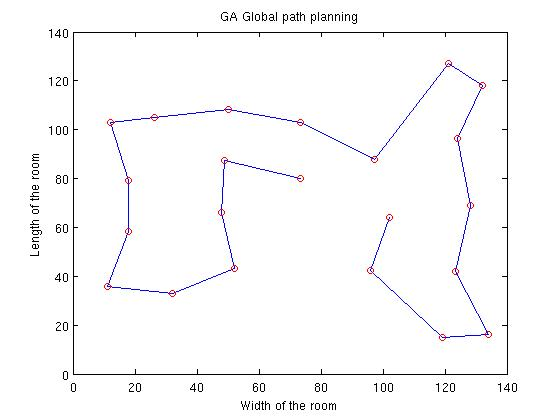
\includegraphics[width=\linewidth]{figures/22pts_GA_linear_2D.jpg}  
  \endminipage \hfill
  \minipage{0.50\textwidth}
  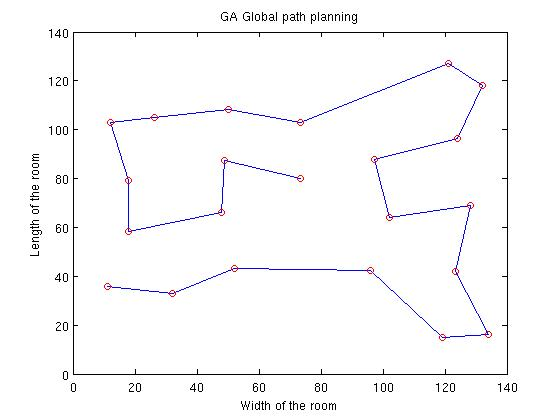
\includegraphics[width=\linewidth]{figures/22pts_GA_linear_2D_2.jpg}  
  \endminipage \hfill
  \caption{GA path planning followed by linear piecewise of 22 waypoints to cover 90.68\% of an area}
  \label{fig:Path_planning}
\end{figure}

The left path length is 511 meters, while the right one is 547 meters for the same area coverage percentage. 

\begin{figure}[H]
\minipage{0.50\textwidth}
  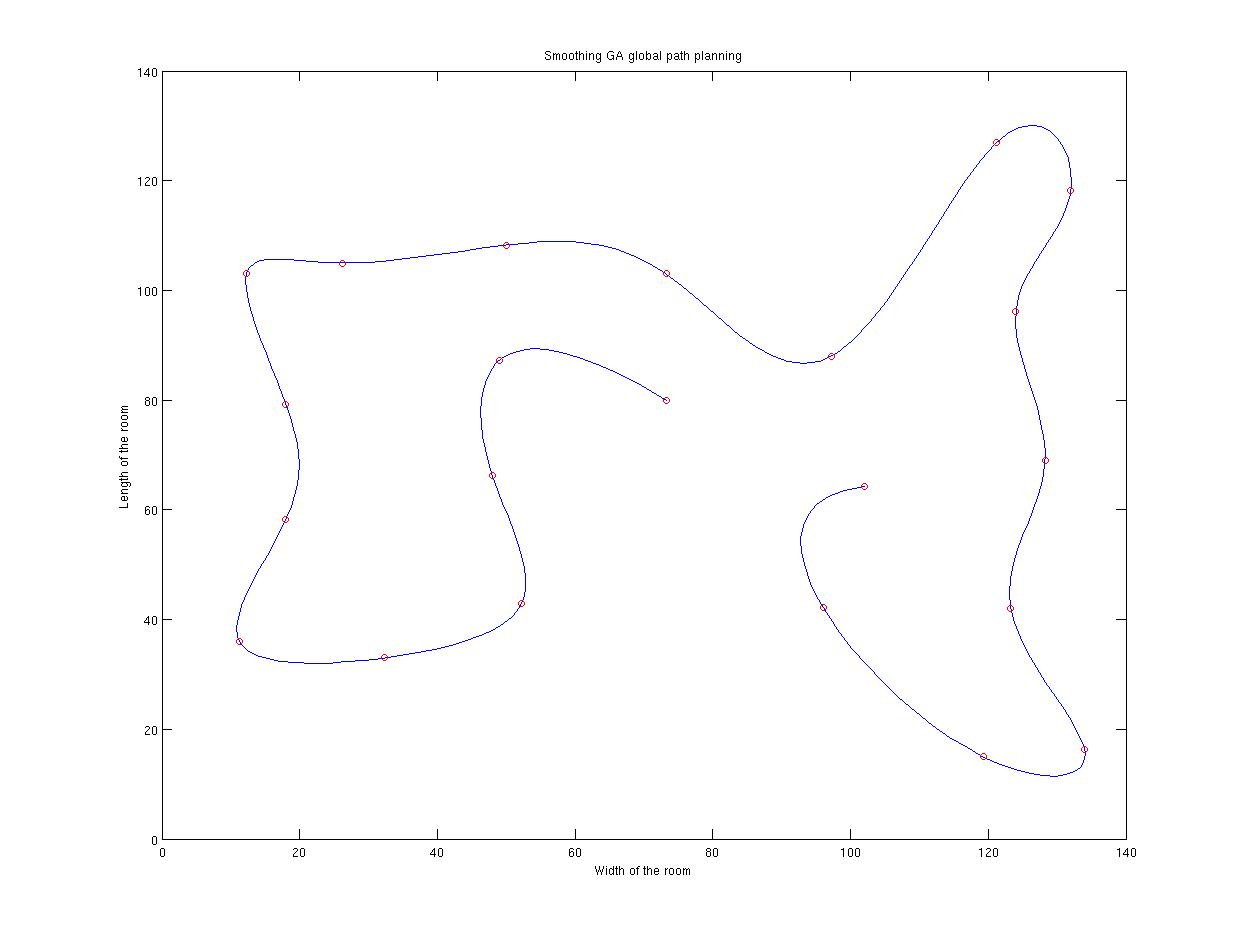
\includegraphics[width=\linewidth]{figures/22pts_GA_linear_2D_1_smooth.jpg}  
  \endminipage \hfill
  \minipage{0.50\textwidth}
  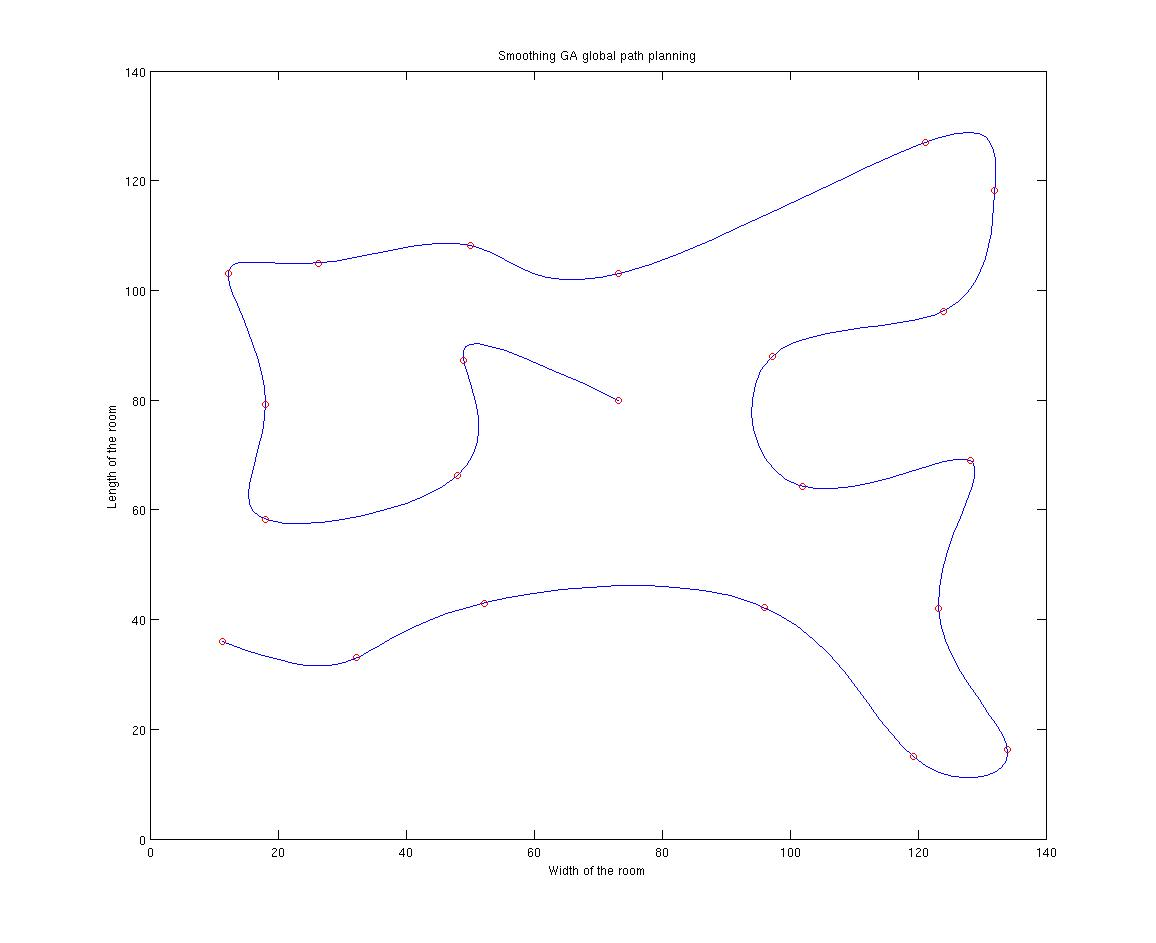
\includegraphics[width=\linewidth]{figures/22pts_GA_linear_2D_2_smooth.jpg}  
  \endminipage \hfill
  
  \caption{Smoothing GA path planning of 22 waypoints to cover 90.68\% of an area}
  \label{fig:smooth_ga_22}
\end{figure}


%   511.9146
% 547
% 558
  

The time elapsed to generate these paths range from 0.475 seconds to 0.507 seconds on a computer with specifications discussed in subsection \ref{computation}

\begin{table}[H]
\centering
\caption{Different results of the path generated by GA}
\label{my-label}
\begin{tabular}{|c|c|c|}
\hline
    Parameter   &  \multicolumn{2}{c|}{Corresponding Values}                 \\ \hline
    Area Coverage    & 79\% & 90.68\%                   \\ \hline
             
           Number of waypoints     & 18 & 22                  \\ \hline
\multirow{4}{*}{Distance in meters} & 486 &  511                 \\ \cline{2-3} 
                 & \multirow{2}{*}{463} & \multirow{3}{*}{547} \\ \cline{2-2} 
                    &  \\ \cline{2-2}
                  & 474 &                   \\ \hline
\end{tabular}
\end{table}

\subsection{Outdoor Simulation Data}
%\textcolor{red}{write about the outdoor a bit }\\
%\textcolor{red}{add the mosaic of the satellite image  in the end}

Aerial map of the laboratoire electronique,informatique et image (LE2I) and its surroundings is captured.  Following to the capture step, comes the discretization of the area. Also blocks covers the areas that are not required to be passed by.

\begin{figure}[H]
\subfigure[Aerial image as seen on map]{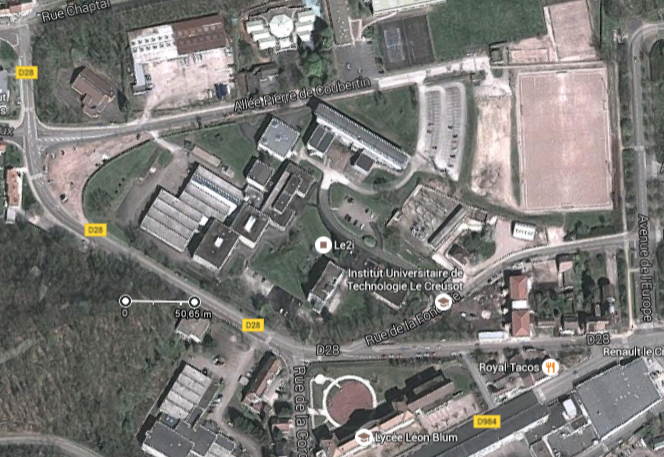
\includegraphics[width=0.54\textwidth]{figures/LE2Imap.PNG}}
\subfigure[unwanted areas to be covered are contoured with rectangles]{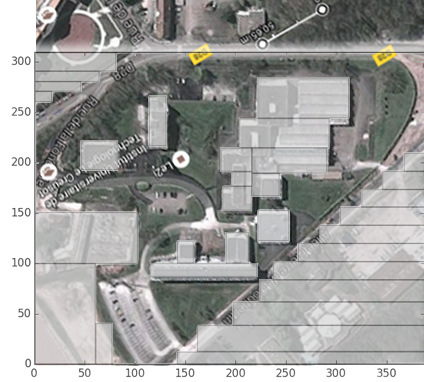
\includegraphics[width=0.45\textwidth]{figures/LE2Imap+wall.jpg}}
\label{pot_field}
  \caption{Aerial Arena }
\end{figure}

\begin{figure}[H]
\minipage{0.45\textwidth}
  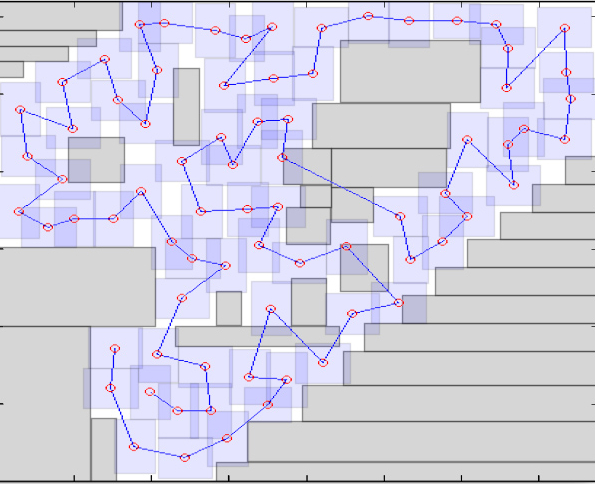
\includegraphics[width=\linewidth]{figures/sattlite_linear.jpg}  
  \endminipage \hfill
  \minipage{0.54\textwidth}
  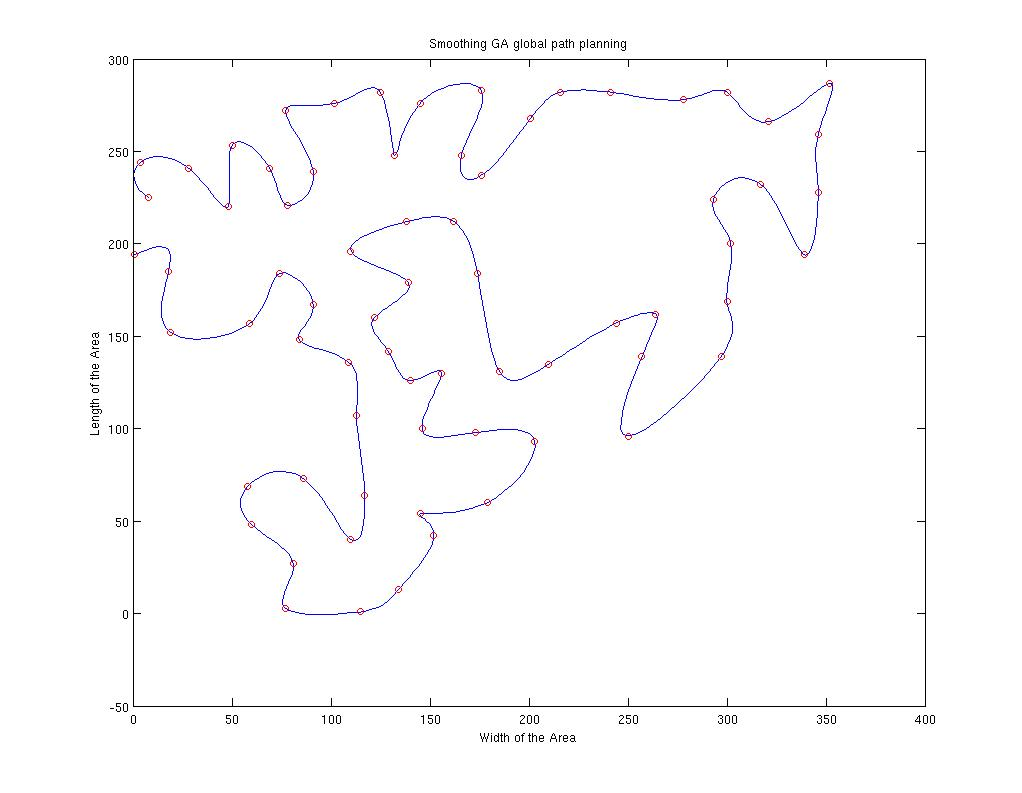
\includegraphics[width=\linewidth]{figures/outdoor_smooth.jpg}  
  \endminipage
  \caption{Imitated area coverage by aerial robot }
  \label{fig:satallite_linear_1}
\end{figure}

Just a reminder that passing over the rectangular blocks is not a forbidden constraint. This area has no interest to be covered, but there is no harm for the robot to pass over it.



\subsection{Artificial Potential Field}
In case of, passing by the unwanted areas became a constraint. Artificial potential field can be a good solution. It is also offering very good results to avoid any appearing obstacles, but with the limitation of falling in local minima.

The context of this experiment is done by picking the waypoint and its consecutive one. Then generate a potential field map and let the robot navigate to it.

The points shown in this experiment are the ones that the linear and spline piecewise shows cutting over the unwanted area to be covered. This solution comes with the price of slightly increasing the length of the coverage path.

\begin{figure}[H]
\centering
 \subfigure[Attractive potential field map]{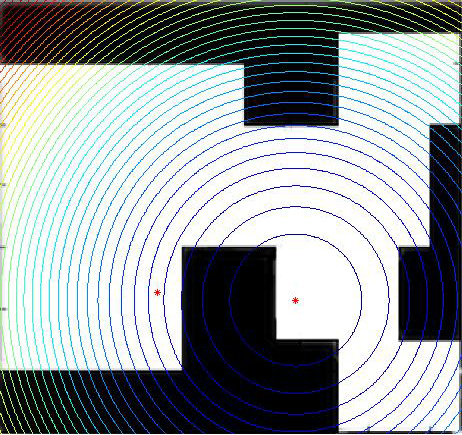
\includegraphics[width=0.49\textwidth]{figures/APF/attractive_pot_field.jpg}
 } \hfill
\subfigure[Repulsive potential field map]{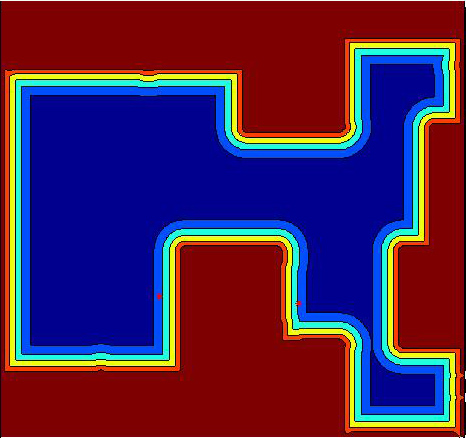
\includegraphics[width=0.49\textwidth]{figures/APF/repulsive_pot_field.jpg}}\\

\subfigure[Summary potential field map]{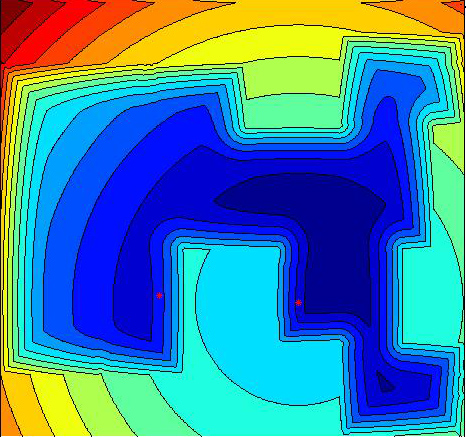
\includegraphics[width=0.45\textwidth]{figures/APF/summary_pot_field.jpg}}
\subfigure[Path from one point to the consecutive]{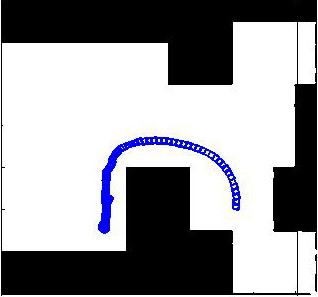
\includegraphics[width=0.45\textwidth]{figures/APF/path_field_better2.jpg}}
\label{pot_field}
  \caption{Potential field map}
\end{figure}

\section{Real World Experiments} \label{real_robot}

\subsection{Quadcopter Hardware}\label{real_robot_hardware}

The Quadcoptor used to do this experiments is an offshelf commercially found drone from the French company Parrot which is AR.drone 2.0. It was first introduced in 2010 as a toy for Augmented Reality games. Shortly research labs, universities make use of its comparably cheap and low weight in their experiments. Hardware and software specification with sample research usage can be found in \cite{Ardrone1,Ardrone2}. Equipped with two cameras; one of them is pointing downwards makes it clearly very useful for the application of area coverage. This camera runs at 60 fps with a resolution of 176 x 144 pixels, covering a field of view of only 47.5$^{\circ}$ x 36.5$^{\circ}$. Concerning the software, there are mobile applications to control the drone for both IOS and Android. SDK is avilable for computer development. The embedded software that is running onboard is not directly accessible, but sending and transmitting data with telnet shell communication channel is possible. Transmitting navigation data and receiving the sensor readings to the drone is done after connecting a workstation computer to it through ad-hoc wireless LAN network. External ROS packages used to control the quadcopter will be discussed in more details in the next subsections.

\begin{figure}[H]
\center
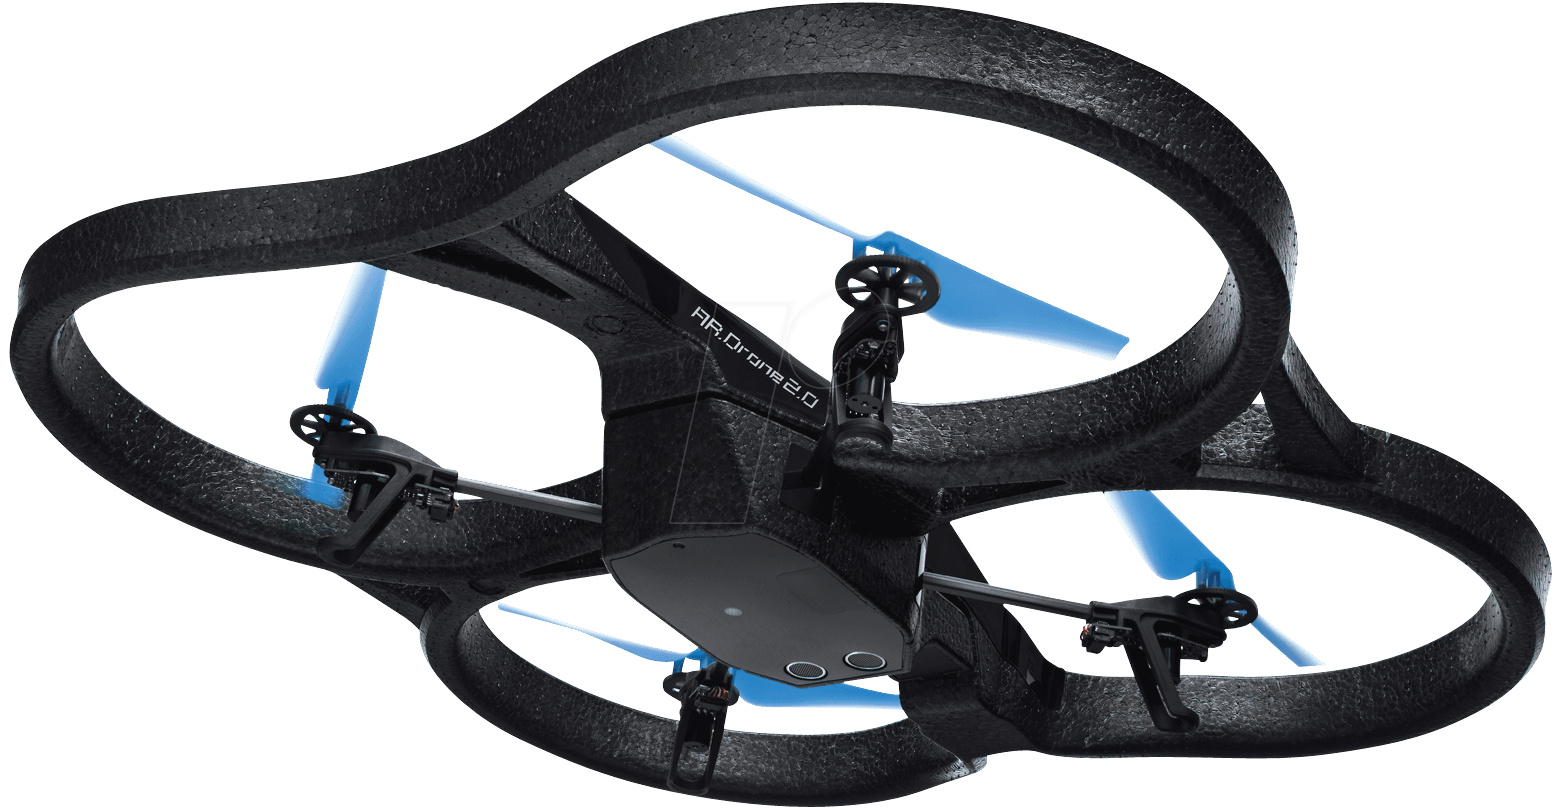
\includegraphics[width=0.49\textwidth]{figures/ar_drone.png}
 \caption{ Ar.Drone 2.0}
 \end{figure}
 
\subsection{Experiment Environment}

As mentioned in \ref{localization_Back} the wide scenarios of generating real experiments with aerial robots, localization problem is crucial. Using the monocular SLAM package developed for AR.Drone by Engel et al. in \cite{engel14ras,engel12iros}  is chosen to solve this challenge. This package proved by practical experimentation its reliability in localizing the robot without any environment modification except putting a panel full of figures to give rich features. Flying arena overview is shown in figure 5.12 .

%\textcolor{red}{put the image of the environment}


\subsection{Robot Localization }

The tum\_ardrone ROS package enables the drone to localize itself  and navigate in an unknown and potentially GPS-denied environments without learning the environment or mapping it previously. Monocular SLAM to compute a visual pose estimate within this map for each video frame. The main contribution of this package is to estimate the scale of map from inertial and altitude measurements by formulating the problem statistically, and deriving a closed-form solution for the maximum likelihood (ML) estimator of the unknown scaling factor. Proportional-integral-differential (PID) control is applied to control the pose of the drone, and fly to and hold a desired target position \cite{engel14ras}.

\subsection{Practical Results}

A plug-in to the tum\_ardrone package is developed for the practical work. This plug-in takes as inputs the waypoints from the path planning module and also the relative position of the drone. The relative position is of the drone current position to the zero position on the map used to generate the path. The plug-in calculates the mid path in between the main waypoints. It is also responsible for toggling the camera of the drone when it reach the waypoints. Then it gives the order of image acquisition.

\begin{figure}[H]
 \subfigure[Drone and flag to be covered]{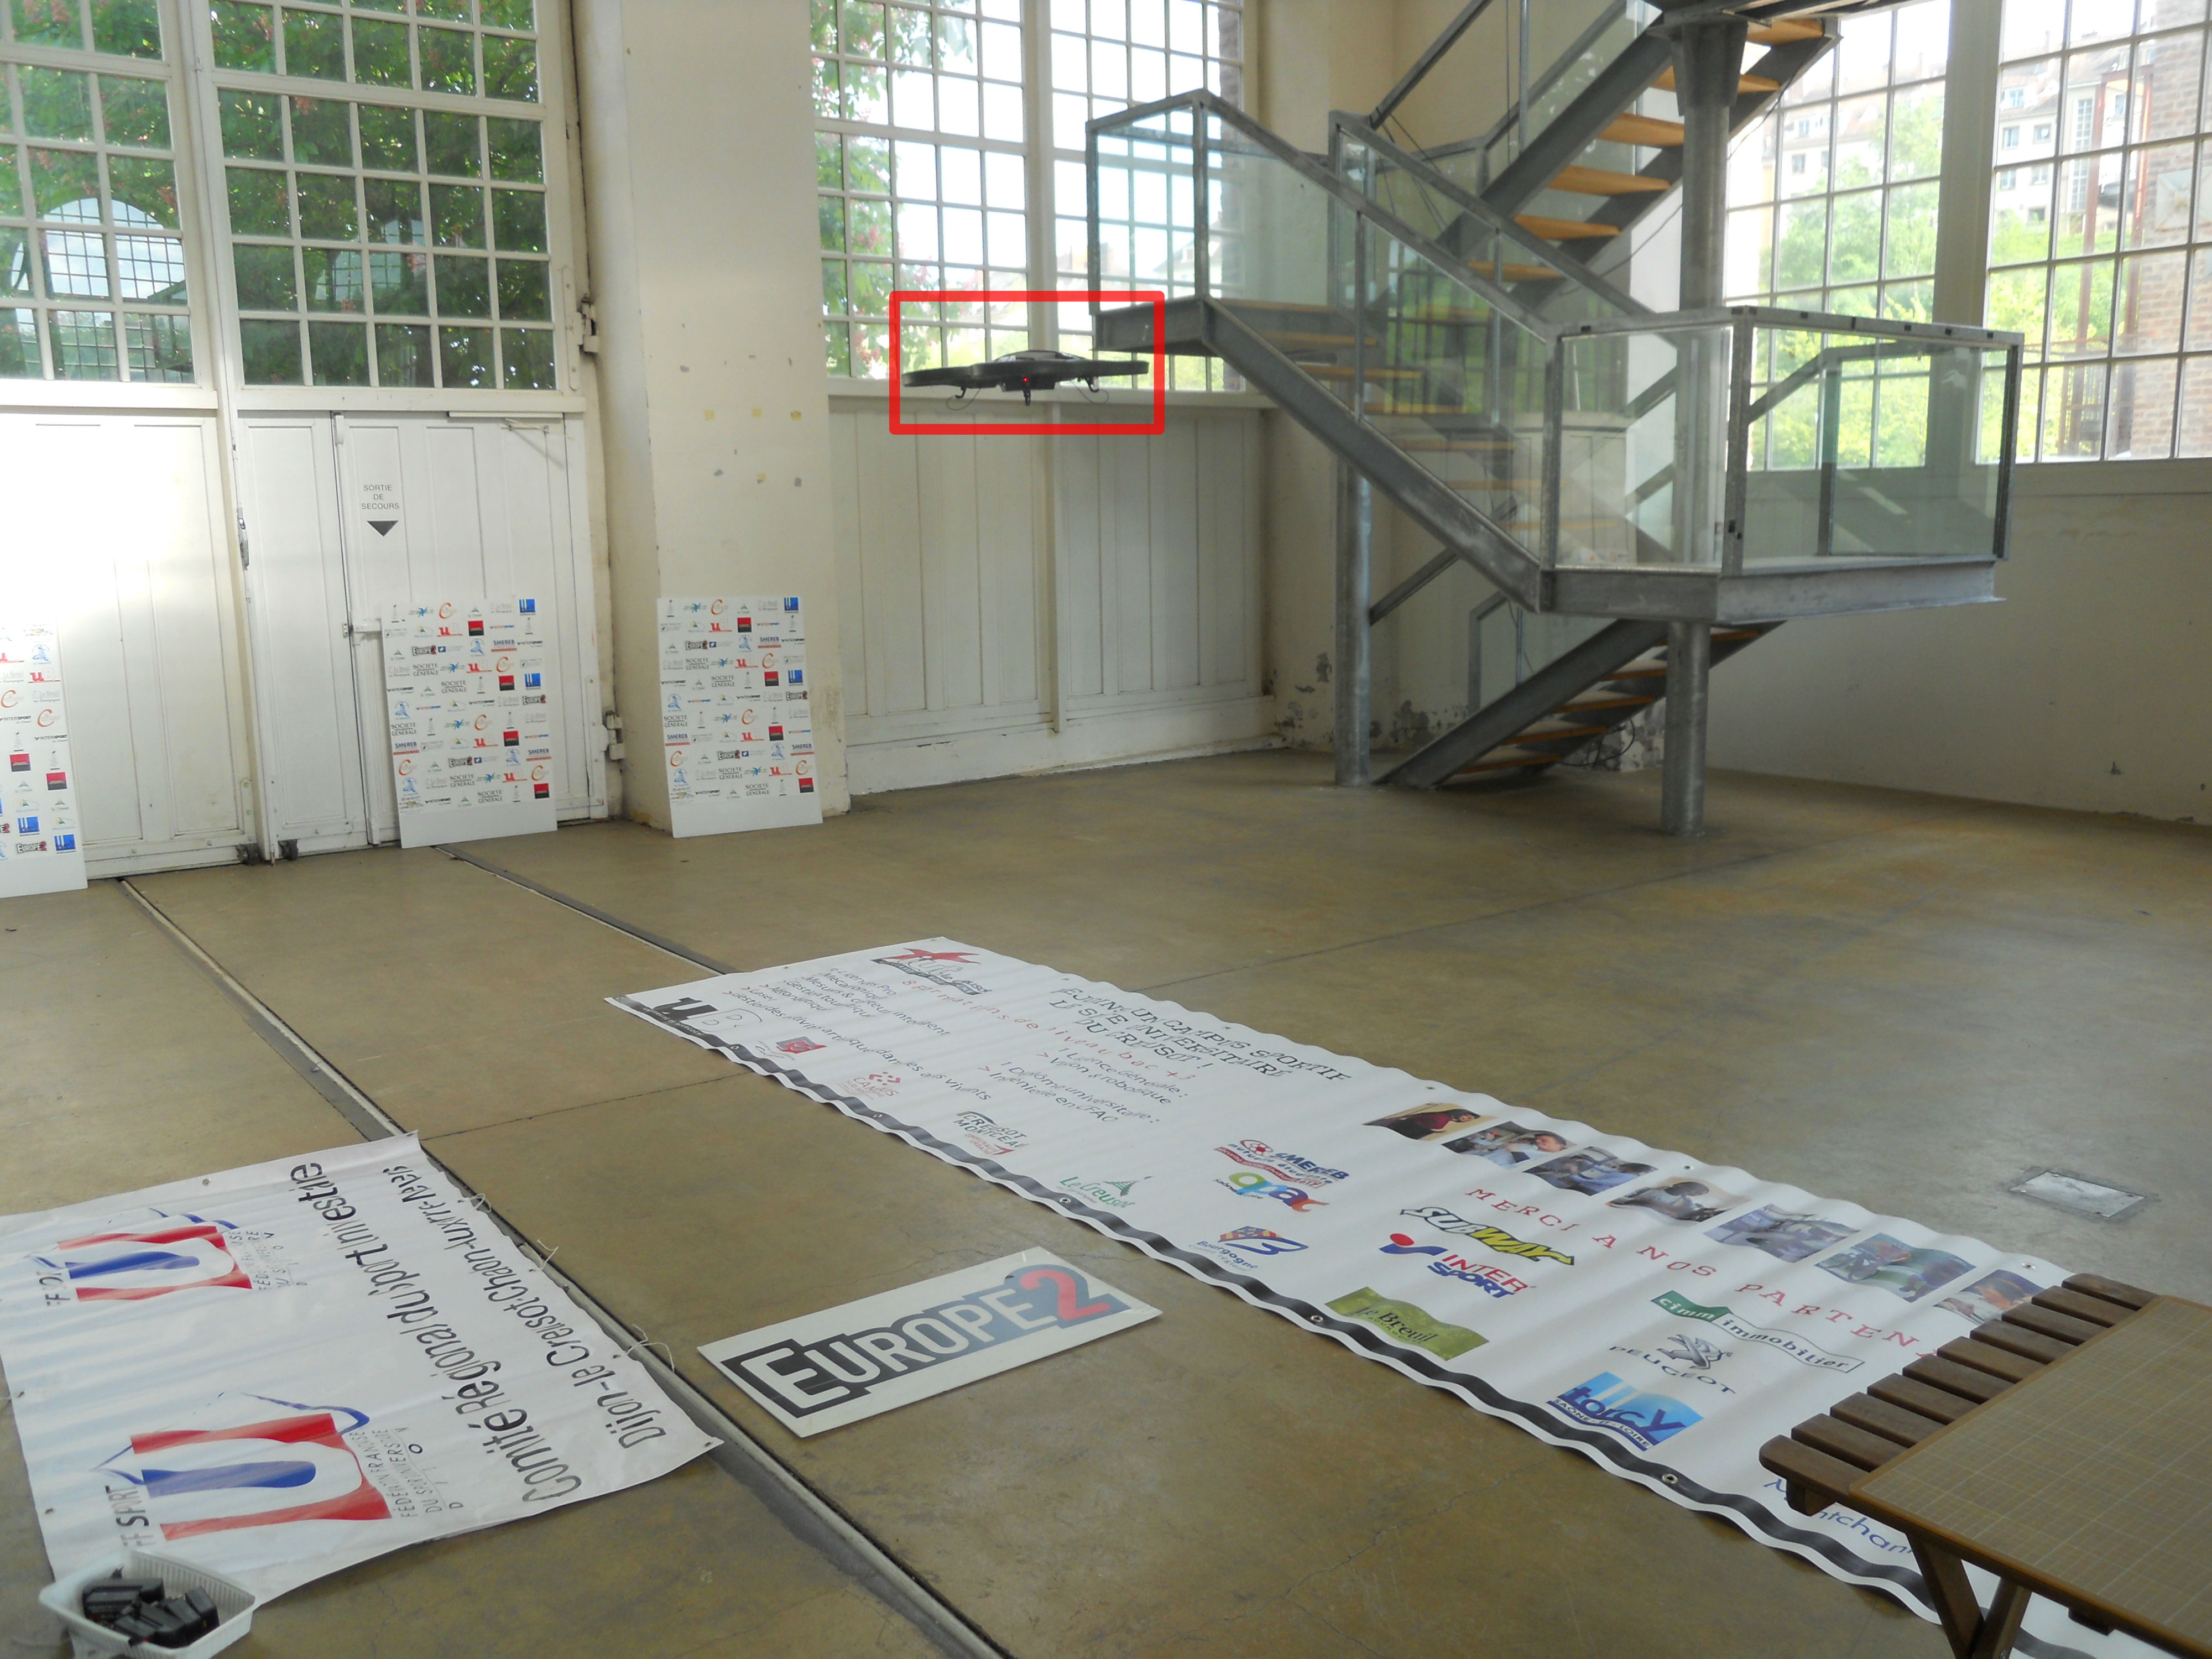
\includegraphics[width=0.45\textwidth]{figures/practical/practical_down.jpg}}
\subfigure[Top view of the flying arena]{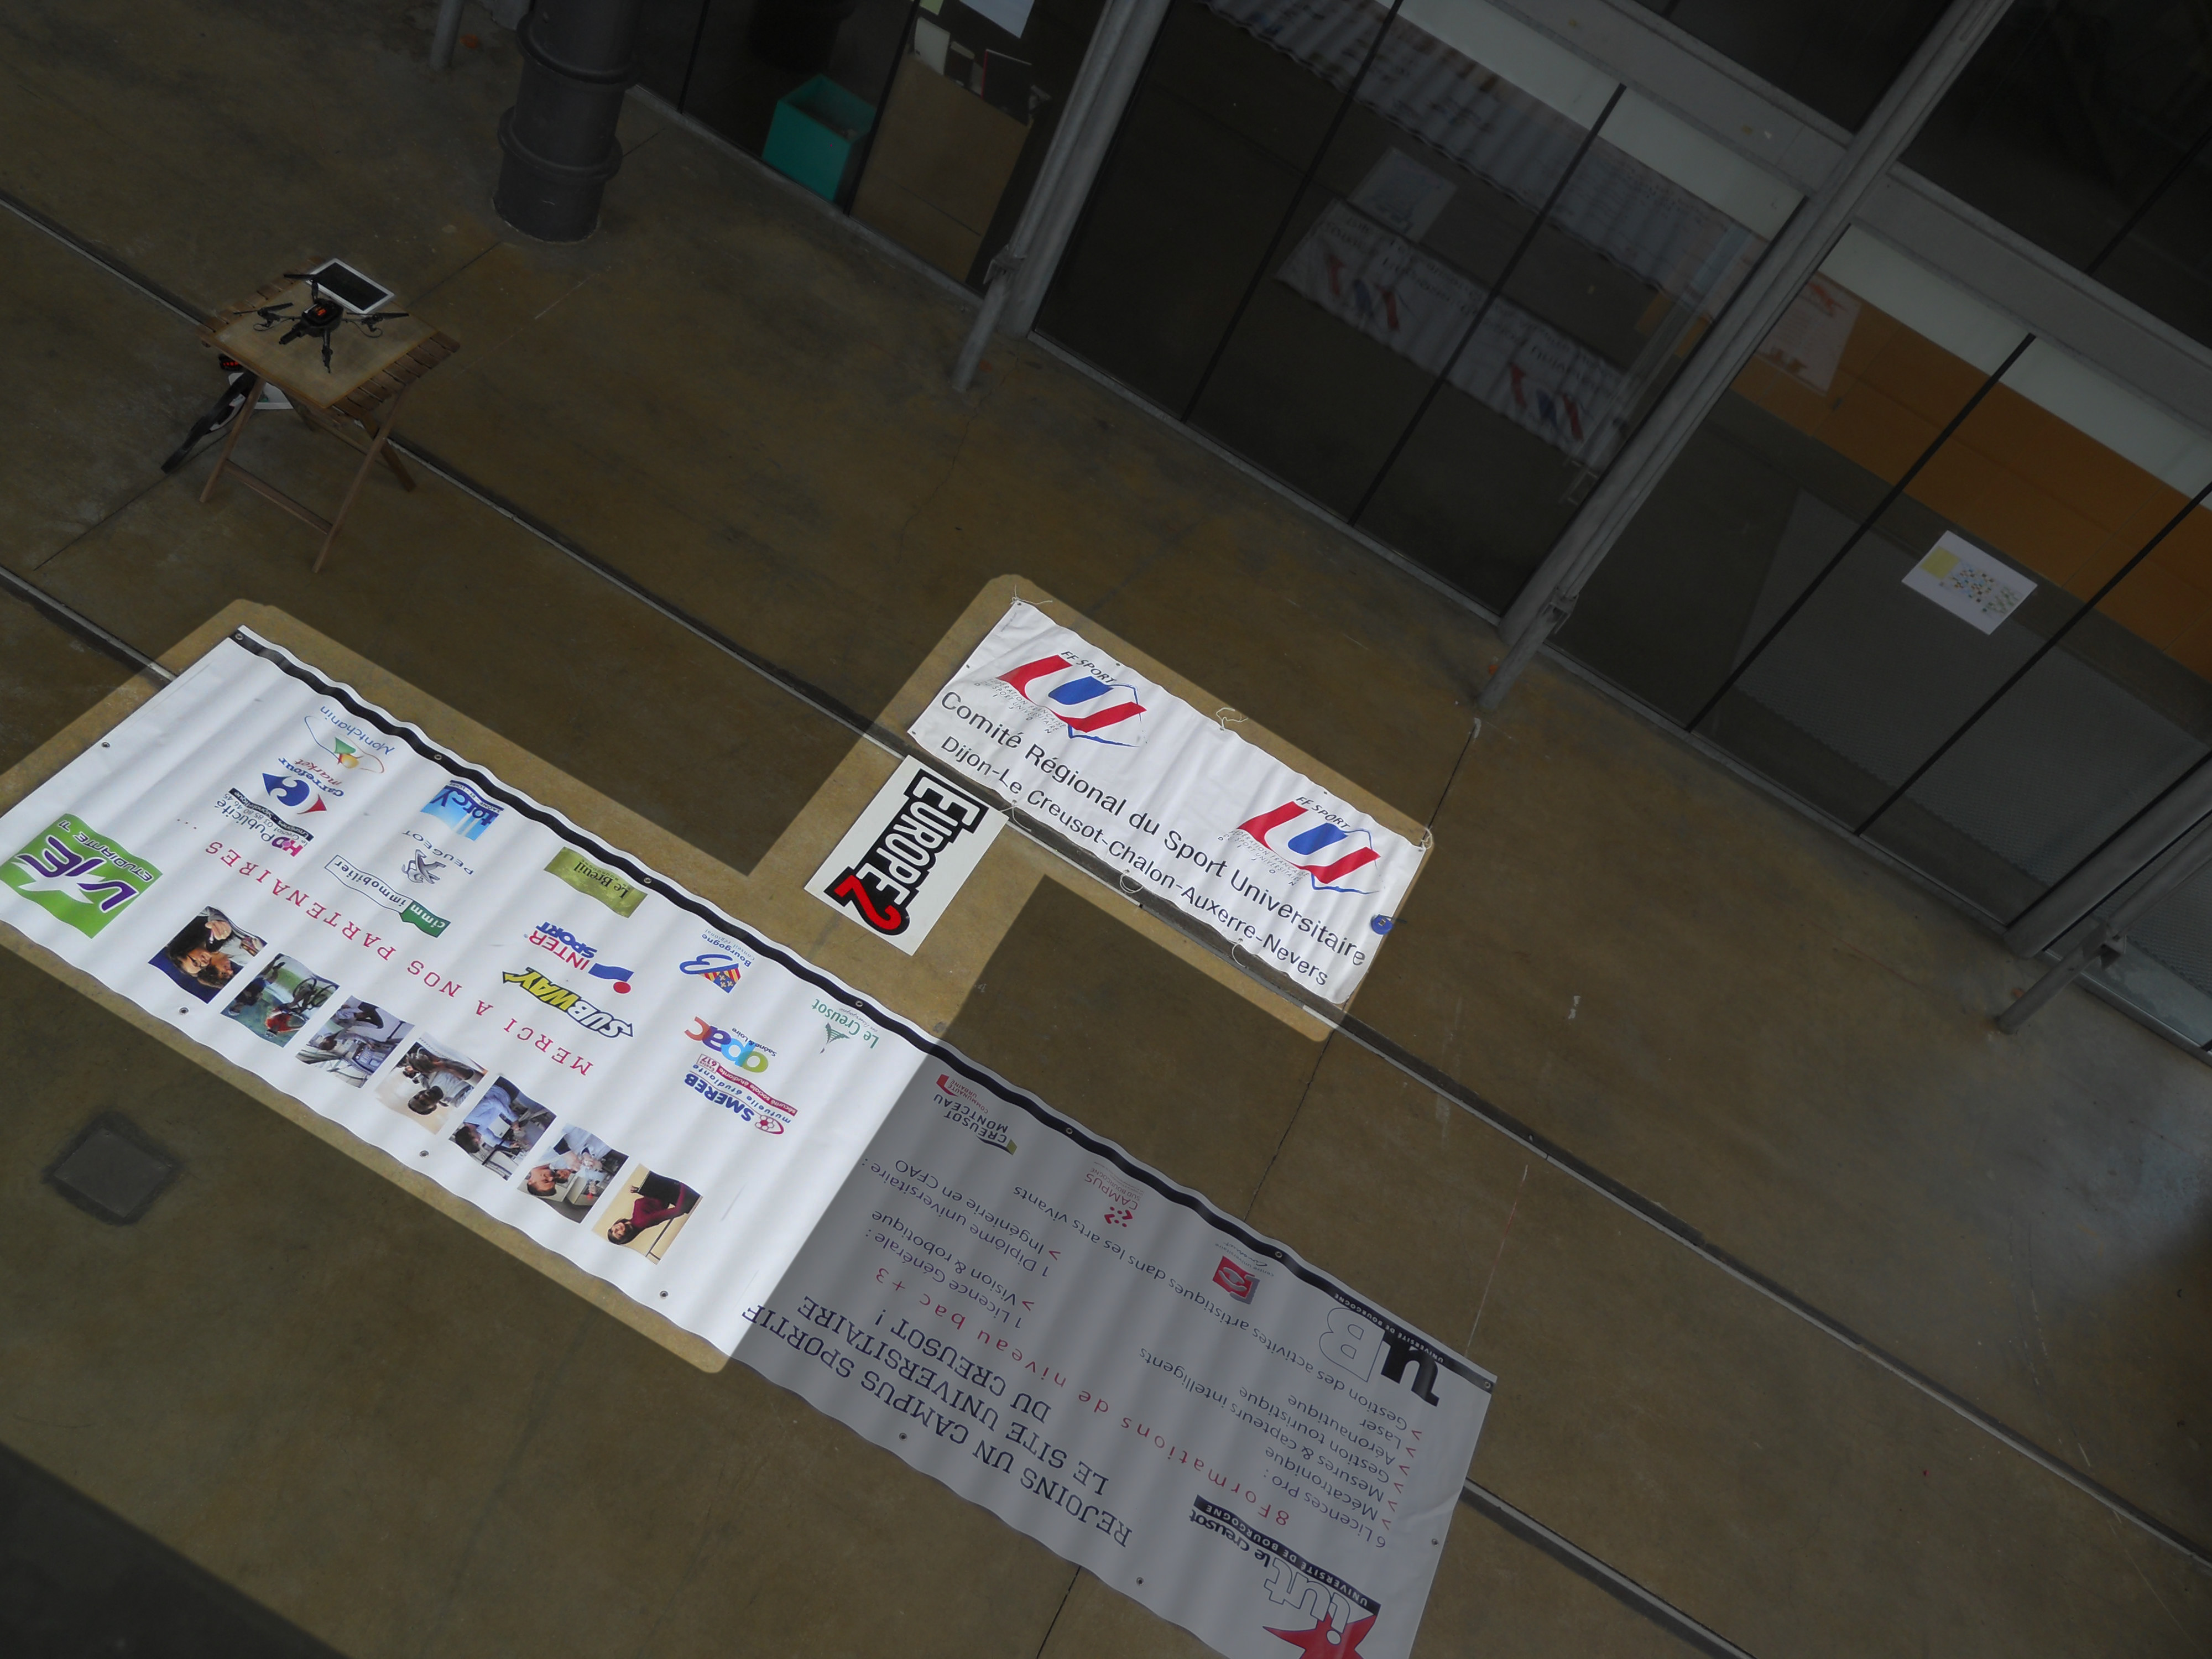
\includegraphics[width=0.45\textwidth]{figures/practical/practical_full_room.jpg}}\label{roomy}
 
  \caption{Workspace for the experiment}
\end{figure}

The highlighted area in figure 5.12 (b) is the area needed to be covered by the robot. Then mosaicking techniques are applied to construct the final image output.

The Path generated from a simulated area that imitate the desired part wanted to be covered.

%This path is then multiplied by a transformation matrix that will translate 

\begin{figure}[H]
 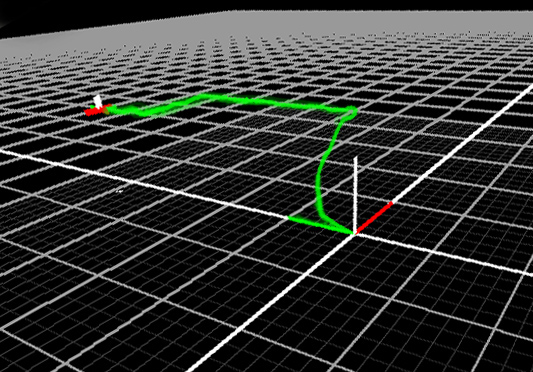
\includegraphics[width=0.75\textwidth]{figures/PTAM_Good2.jpg}
  \caption{Path Planning visualization on PTAM}
\end{figure}
A video showing the robot navigation, path execution, frontal camera scene and mosaicking generation; can be found in this link \cite{mosaic_image_intro}.  
% http://nschloe.blogspot.fr/2009/06/bibtex-how-to-cite-website_21.html
% Odometry Pose Estimation: The “Pose Estimator” is explained in the following article and Master’s Thesis [23], [22]. To correct the drift that the Odometry Pose Estimator module has, absolute measures provided by visual features are used.
 
\section{Mosaicking}

\subsection{Simulation}

The ortho-mosaicked output image composed by the captured
images is very close to a complete top view of the desired area to be covered. Mosaicking in our case is simply computed using the position and orientation coordinates of the known waypoint. Then stitch the images together to validate the optimum choice of the positions where the drone captured these images as shown in Fig.\ref{fig:final_room} for the simulated room in V-REP.

Otho-mosaicking also proved its validity in mosaicking aerial outdoor images as mentioned by Yahyanejad in  \cite{yahyanejad2010incremental}.

The coverage threshold rate is 90\% of the useful area in the room without taking the red block parts into consideration to cover.

\begin{figure}[H]
 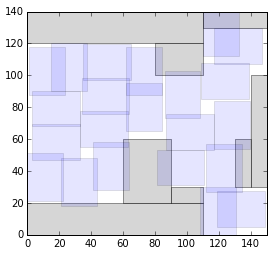
\includegraphics[width=0.45\textwidth,angle=90]{figures/room_python.PNG}
  \caption{Poses of every image captured in the room}
\end{figure}


\begin{figure}[H]
  \centering
  \subfigure[Room mosaicing]{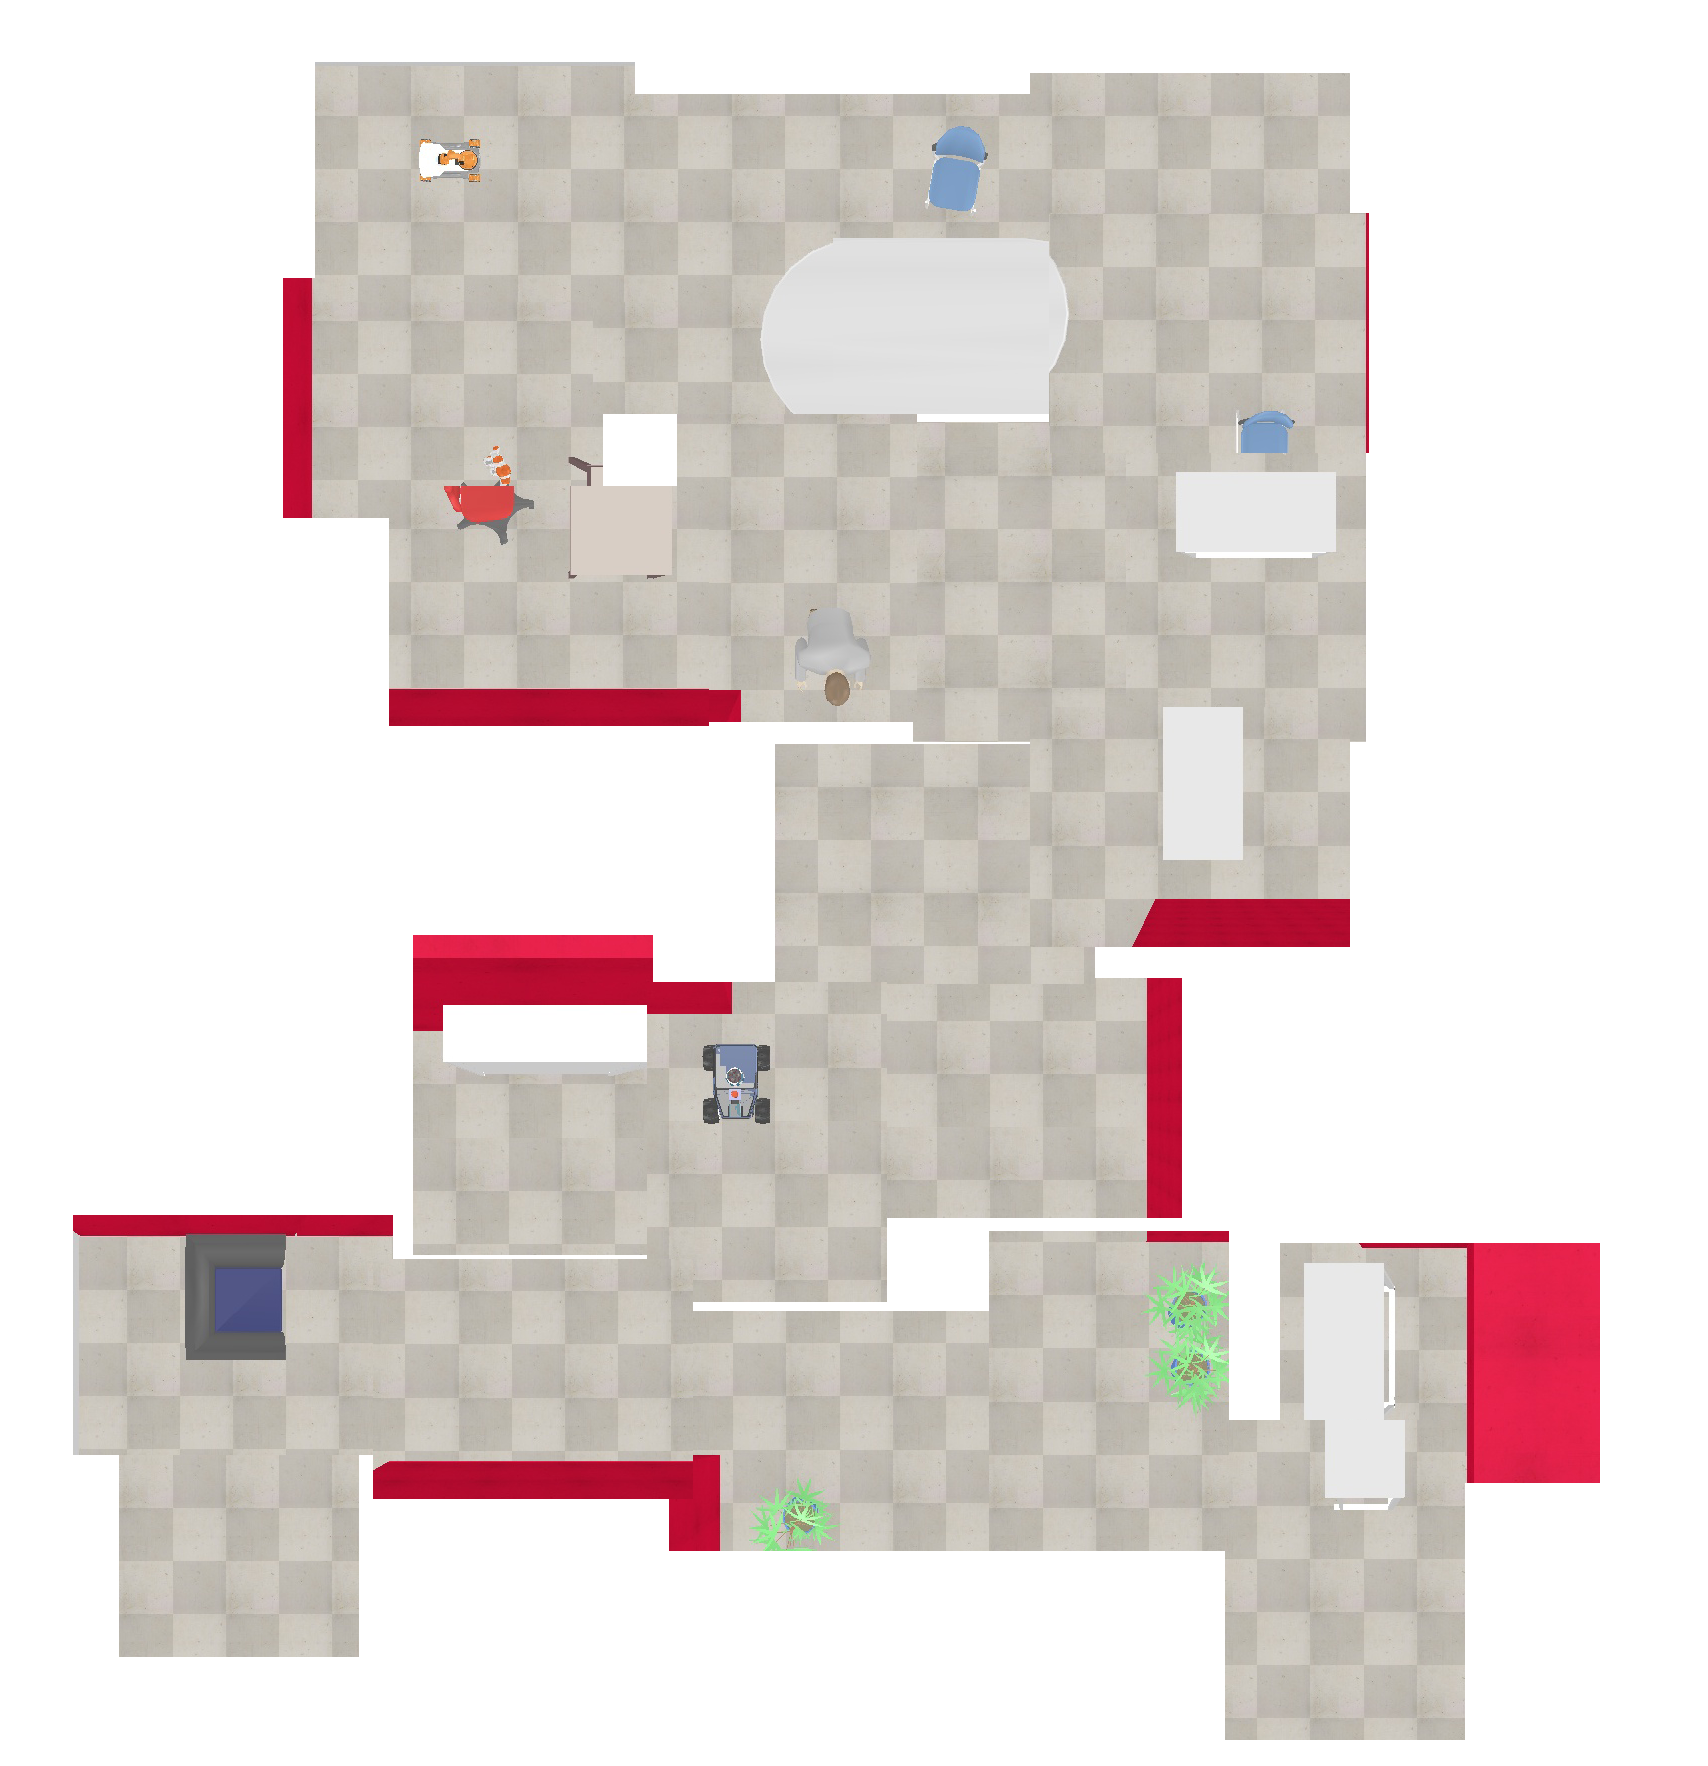
\includegraphics[width=0.45\textwidth,angle=180]{figures/mosaic2.png}}
  \hfill
  \subfigure[Top view of the Room]{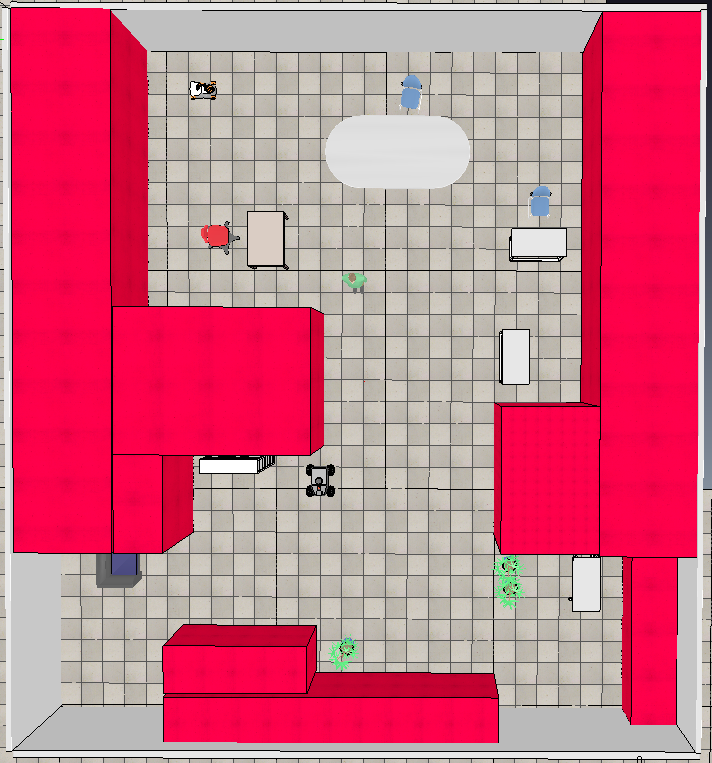
\includegraphics[width=0.45\textwidth,angle=180]{figures/room_full2.png}}
  \caption{Room Coverage}
  
  \label{fig:final_room}
  
\end{figure}




\subsection{Practical}
The mosaicking process of the practical experiment is done after the flight. The acquired images used to generate the figure \ref{fig:mosaic_practical} are 32 images. The several image on the same waypoint is shoot, so that the images with best correspondences will be used. This result is not by the mosaic developed by the author for the simulation. Indeed it is done by a well known software online; provided by Microsoft Research for free of use. It is called Image Composite Editor.

\begin{figure}[H]
  \centering
  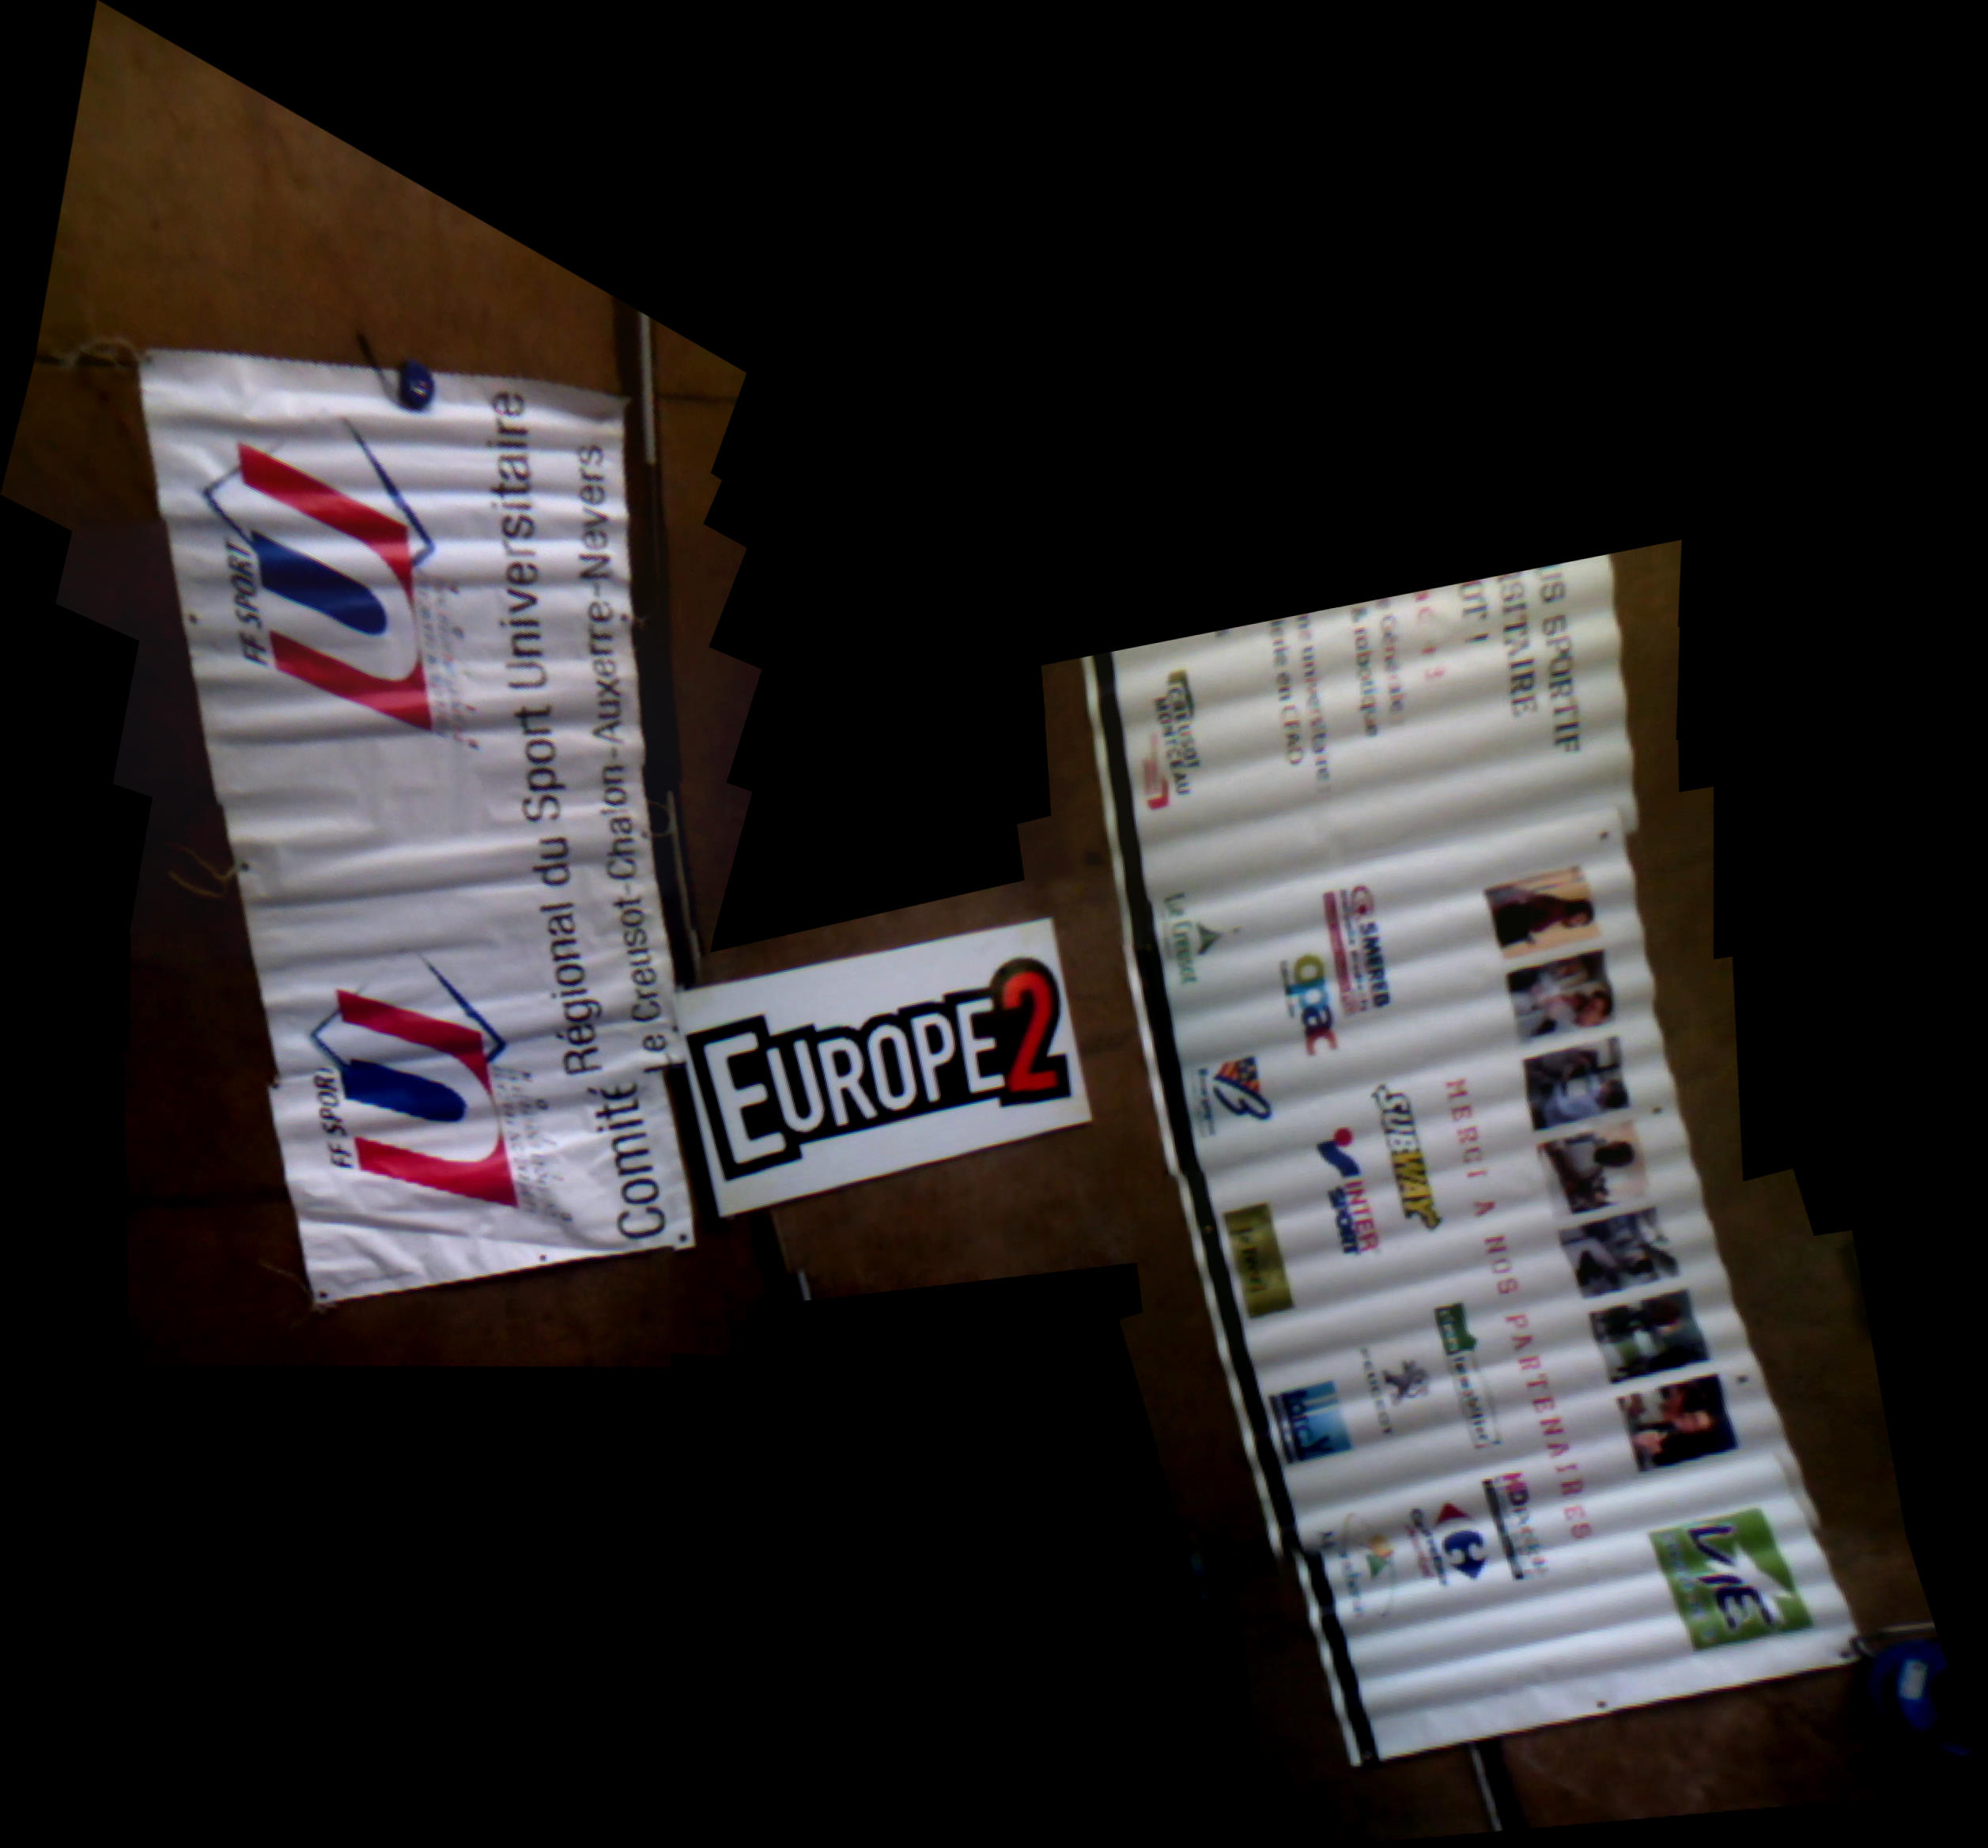
\includegraphics[width=0.65\textwidth]{figures/practical/mosaic_practical.jpg}
  
  \caption{Flags Mosiacing}
  
  \label{fig:mosaic_practical}
  
\end{figure}


\section{Computation} \label{computation}
The computer used to generate these experiments is specified with 8 GB of memory (RAM). Processor is Intel® Core™ i7-2720QM CPU @ 2.20GHz ×8. 
The OS is ubuntu 14.04 LTS. Codes developed is developed by C++11, python 2, Matlab 2013B. V-REP version is 3.3.x. The ROS package is tested on ROS distribution Indigo.